\documentclass[a4paper, 11pt]{article}
%%%%%%%%%%%%%%%%%%%%%%%%%%%%%%%%%%%%%%%%%%%%%%%%%%%%%
%						Packages					%
%%%%%%%%%%%%%%%%%%%%%%%%%%%%%%%%%%%%%%%%%%%%%%%%%%%%%
\usepackage{latexsym,amsfonts, amsmath, amssymb, amsthm}
% \usepackage{mathpazo}
\usepackage[utf8]{inputenc}
\usepackage[final=true,protrusion=true,expansion=true]{microtype}
\usepackage[noadjust]{cite}
\usepackage{enumitem}
\usepackage{color}
\usepackage{mathtools}

% Table
\usepackage{booktabs}
\usepackage{multirow}

\usepackage{subcaption}
\usepackage[font=scriptsize,labelfont=bf]{caption}
\usepackage[affil-it]{authblk}

%
% Margins
\usepackage{geometry}
\geometry{
a4paper,
total={160mm,247mm},
left=22mm,
right=22mm,
top=20mm,
}

% Href
\usepackage{hyperref}
\hypersetup{
	final,
    colorlinks=true,
    linkcolor=blue,
    filecolor=magenta,
    urlcolor=cyan,
}

%%%%%%%%%%%%%%%%%%%%%%%%%%%%%%%%%%%%%%%%%%%%%%%%%%%%%
%					Theorem Styles					%
%%%%%%%%%%%%%%%%%%%%%%%%%%%%%%%%%%%%%%%%%%%%%%%%%%%%%
\theoremstyle{plain}
\newtheorem{theorem}{Theorem}
\newtheorem{proposition}[theorem]{Proposition}
\newtheorem{lemma}[theorem]{Lemma}
\newtheorem{corollary}[theorem]{Corollary}
\newtheorem{claim}[theorem]{Claim}
\newtheorem{problem}{Problem}

\theoremstyle{plain}
\newtheorem{definition}[theorem]{Definition}
\newtheorem{example}[theorem]{Example}
\newtheorem{remark}[theorem]{Remark}

%======================================================================
% MACROS
% ======================================================================
\providecommand*{\Covv}[1]{\operatorname{Cov}\left({#1}\right)}   % distance
\providecommand*{\textCovv}[1]{\operatorname{Cov}({#1})}   % distance

\providecommand*{\Covvn}[2]{\operatorname{Cov}_{#2}\left({#1}\right)}   % distance
\providecommand*{\Var}[1]{\operatorname{Var}\left({#1}\right)}   % distance
\providecommand*{\textVar}[1]{\operatorname{Var}({#1})}   % distance

\providecommand*{\Uni}[1]{\operatorname{Uni}({#1})}
\providecommand*{\Span}{\operatorname{span}}     % Span

% distance
\providecommand*{\len}[1]{\operatorname{length}({#1})}   % distance
\providecommand{\subG}{\operatorname{subG}}
\providecommand*{\seqInt}[2]{[{#1}:{#2}]}   %
% Operators

\providecommand{\Bdsymb}{\Gamma}                   % Tag for boundary operators
\providecommand{\Div}{\operatorname{div}}          % Divergence
\providecommand{\bDiv}{{\Div}_{\Bdsymb}}           % Surface divergence
\providecommand{\mDiv}{\operatorname{\sf div}}     % matrix divergence
\providecommand{\curl}{\operatorname{{\bf curl}}}  % Standard curl operator
\providecommand{\plcurl}{\operatorname{{\bf curl}}_{2D}} % Vectorial curl operator in 2D
\providecommand{\bcurl}{{\curl}_{\Bdsymb}}         % vectorial curl on the surface
\providecommand{\bscurl}{\operatorname{curl}_{\Bdsymb}} % scalar curl on a surface
\providecommand{\scurl}{\operatorname{curl}_{2D}}       % scalar curl in 2D
\providecommand{\mcurl}{\operatorname{{\bf\sf curl}}}   % matrix curl operator
\providecommand{\grad}{\operatorname{{\bf grad}}}       % standard gradient
\providecommand{\bgrad}{\grad_{\Bdsymb}}                % Surface gradient
\providecommand{\mgrad}{\operatorname{{\bf\sf grad}}}   % Matrix gradient for row vectors

\providecommand{\Dim}{\operatorname{dim}}            % dimension
\providecommand{\dim}{\Dim}
\providecommand{\Card}{\sharp}                       % numel of a set (cardinality)
\providecommand{\Vol}{\operatorname{Vol}}   % volume
\providecommand{\vol}{\Vol}
\providecommand{\ker}{\operatorname{ker}}
\providecommand{\ran}{\operatorname{ran}}
\providecommand*{\Meas}[2][]{\operatorname{meas}_{#1}({#2})} % measure
\providecommand*{\meas}[2][]{\Meas{#1}{#2}}
\providecommand*{\dist}[2]{\operatorname{dist}({#1};{#2})}   % distance
\providecommand*{\normaldist}[2]{\operatorname{ndist}({#1};{#2})}   % distance
\providecommand*{\Dist}[2]{\dist{#1}{#2}}
\providecommand{\Det}{\operatorname{det}}                    % determinant
\providecommand{\Sgn}{\operatorname{sgn}}                    % sign
\providecommand*{\Kern}[1]{{\rm Ker}({#1})}                  % Kernel
\providecommand*{\Dom}[1]{{\rm Dom}({#1})}                   % Domain
\providecommand*{\Span}[1]{\operatorname{Span}\left\{{#1}\right\}}     % Span
\providecommand*{\Convex}[1]{\operatorname{convex}\left\{{#1}\right\}} % convex hull
\providecommand{\Supp}{\operatorname{supp}}                            % support
\providecommand{\supp}{\Supp}
\providecommand{\WF}{\operatorname{WF}}                            % wavefront se

%\providecommand{\dist}{\operatorname{dist}}                        % rank

\providecommand{\sing}{\operatorname{sing}}                            % support
\providecommand*{\Image}[1]{\mathrm{Im}({#1})}                         % Image
\providecommand*{\Range}[1]{\operatorname{Range}({#1})}                % Range
\providecommand{\range}{\operatorname{range}}                % Range
\providecommand{\rank}{\operatorname{rank}}                        % rank
\providecommand{\Rank}{\rank}
\renewcommand{\Re}{\operatorname{Re}}             % real part
\renewcommand{\Im}{\operatorname{Im}}             % imaginary part
\providecommand{\argmin}{\operatorname*{\arg\min}}  % argument yielding inf
\providecommand{\arginf}{\operatorname*{arginf}}  % argument yielding inf
\providecommand{\argmax}{\operatorname*{argmax}}  % argument yielding max
\providecommand{\nnz}{\operatorname{nnz}}         % no of nonzeros
\providecommand{\Id}{\Op{Id}}                     % Identity operator
\providecommand{\diam}{\operatorname{diam}}
\providecommand{\diag}{\operatorname{diag}}
\providecommand{\Diag}[1]{\operatorname{Diag}\left({#1}\right)}
\providecommand{\esssup}{\operatorname*{esssup}}
\providecommand{\essinf}{\operatorname*{essinf}}
\providecommand{\limsup}{\operatorname*{limsup}}
\providecommand{\closed}[1]{\operatorname*{cl}\left({#1}\right)}


% Bold small letters (for vectors)

\newcommand{\Va}{{\mathbf{a}}}
\newcommand{\Vb}{{\mathbf{b}}}
\newcommand{\Vc}{{\mathbf{c}}}
\newcommand{\Vd}{{\mathbf{d}}}
\newcommand{\Ve}{{\mathbf{e}}}
\newcommand{\Vf}{{\mathbf{f}}}
\newcommand{\Vg}{{\mathbf{g}}}
\newcommand{\Vh}{{\mathbf{h}}}
\newcommand{\Vi}{{\mathbf{i}}}
\newcommand{\Vj}{{\mathbf{j}}}
\newcommand{\Vk}{{\mathbf{k}}}
\newcommand{\Vl}{{\mathbf{l}}}
\newcommand{\Vm}{{\mathbf{m}}}
\newcommand{\Vn}{{\mathbf{n}}}
\newcommand{\Vo}{{\mathbf{o}}}
\newcommand{\Vp}{{\mathbf{p}}}
\newcommand{\Vq}{{\mathbf{q}}}
\newcommand{\Vr}{{\mathbf{r}}}
\newcommand{\Vs}{{\mathbf{s}}}
\newcommand{\Vt}{{\mathbf{t}}}
\newcommand{\Vu}{{\mathbf{u}}}
\newcommand{\Vv}{{\mathbf{v}}}
\newcommand{\Vw}{{\mathbf{w}}}
\newcommand{\Vx}{{\mathbf{x}}}
\newcommand{\Vy}{{\mathbf{y}}}
\newcommand{\Vz}{{\mathbf{z}}}

% Small bold math characters

\providecommand{\Ba}{{\boldsymbol{a}}}
\providecommand{\Bb}{{\boldsymbol{b}}}
\providecommand{\Bc}{{\boldsymbol{c}}}
\providecommand{\Bd}{{\boldsymbol{d}}}
\providecommand{\Be}{{\boldsymbol{e}}}
\providecommand{\Bf}{{\boldsymbol{f}}}
\providecommand{\Bg}{{\boldsymbol{g}}}
\providecommand{\Bh}{{\boldsymbol{h}}}
\providecommand{\Bi}{{\boldsymbol{i}}}
\providecommand{\Bj}{{\boldsymbol{j}}}
\providecommand{\Bk}{{\boldsymbol{k}}}
\providecommand{\Bl}{{\boldsymbol{l}}}
\providecommand{\Bm}{{\boldsymbol{m}}}
\providecommand{\Bn}{{\boldsymbol{n}}}
\providecommand{\Bo}{{\boldsymbol{o}}}
\providecommand{\Bp}{{\boldsymbol{p}}}
\providecommand{\Bq}{{\boldsymbol{q}}}
\providecommand{\Br}{{\boldsymbol{r}}}
\providecommand{\Bs}{{\boldsymbol{s}}}
\providecommand{\Bt}{{\boldsymbol{t}}}
\providecommand{\Bu}{{\boldsymbol{u}}}
\providecommand{\Bv}{{\boldsymbol{v}}}
\providecommand{\Bw}{{\boldsymbol{w}}}
\providecommand{\Bx}{{\boldsymbol{x}}}
\providecommand{\By}{{\boldsymbol{y}}}
\providecommand{\Bz}{{\boldsymbol{z}}}

% Capital bold Characters

\newcommand{\VA}{{\mathbf{A}}}
\newcommand{\VB}{{\mathbf{B}}}
\newcommand{\VC}{{\mathbf{C}}}
\newcommand{\VD}{{\mathbf{D}}}
\newcommand{\VE}{{\mathbf{E}}}
\newcommand{\VF}{{\mathbf{F}}}
\newcommand{\VG}{{\mathbf{G}}}
\newcommand{\VH}{{\mathbf{H}}}
\newcommand{\VI}{{\mathbf{I}}}
\newcommand{\VJ}{{\mathbf{J}}}
\newcommand{\VK}{{\mathbf{K}}}
\newcommand{\VL}{{\mathbf{L}}}
\newcommand{\VM}{{\mathbf{M}}}
\newcommand{\VN}{{\mathbf{N}}}
\newcommand{\VO}{{\mathbf{O}}}
\newcommand{\VP}{{\mathbf{P}}}
\newcommand{\VQ}{{\mathbf{Q}}}
\newcommand{\VR}{{\mathbf{R}}}
\newcommand{\VS}{{\mathbf{S}}}
\newcommand{\VT}{{\mathbf{T}}}
\newcommand{\VU}{{\mathbf{U}}}
\newcommand{\VV}{{\mathbf{V}}}
\newcommand{\VW}{{\mathbf{W}}}
\newcommand{\VX}{{\mathbf{X}}}
\newcommand{\VY}{{\mathbf{Y}}}
\newcommand{\VZ}{{\mathbf{Z}}}

% Capital bold characters in math mode

\providecommand{\BA}{{\boldsymbol{A}}}
\providecommand{\BB}{{\boldsymbol{B}}}
\providecommand{\BC}{{\boldsymbol{C}}}
\providecommand{\BD}{{\boldsymbol{D}}}
\providecommand{\BE}{{\boldsymbol{E}}}
\providecommand{\BF}{{\boldsymbol{F}}}
\providecommand{\BG}{{\boldsymbol{G}}}
\providecommand{\BH}{{\boldsymbol{H}}}
\providecommand{\BI}{{\boldsymbol{I}}}
\providecommand{\BJ}{{\boldsymbol{J}}}
\providecommand{\BK}{{\boldsymbol{K}}}
\providecommand{\BL}{{\boldsymbol{L}}}
\providecommand{\BM}{{\boldsymbol{M}}}
\providecommand{\BN}{{\boldsymbol{N}}}
\providecommand{\BO}{{\boldsymbol{O}}}
\providecommand{\BP}{{\boldsymbol{P}}}
\providecommand{\BQ}{{\boldsymbol{Q}}}
\providecommand{\BR}{{\boldsymbol{R}}}
\providecommand{\BS}{{\boldsymbol{S}}}
\providecommand{\BT}{{\boldsymbol{T}}}
\providecommand{\BU}{{\boldsymbol{U}}}
\providecommand{\BV}{{\boldsymbol{V}}}
\providecommand{\BW}{{\boldsymbol{W}}}
\providecommand{\BX}{{\boldsymbol{X}}}
\providecommand{\BY}{{\boldsymbol{Y}}}
\providecommand{\BZ}{{\boldsymbol{Z}}}

\newcommand{\nablabf}{\boldsymbol{\nabla}}
\newcommand{\alphabf}{\boldsymbol{\alpha}}
\newcommand{\betabf}{\boldsymbol{\beta}}
\newcommand{\gammabf}{\boldsymbol{\gamma}}
\newcommand{\deltabf}{\boldsymbol{\delta}}
\newcommand{\epsilonbf}{\boldsymbol{\epsilon}}
\newcommand{\varepsilonbf}{\boldsymbol{\varepsilon}}
\newcommand{\zetabf}{\boldsymbol{\zeta}}
\newcommand{\etabf}{\boldsymbol{\eta}}
\newcommand{\thetabf}{\boldsymbol{\theta}}
\newcommand{\varthetabf}{\boldsymbol{\vartheta}}
\newcommand{\iotabf}{\boldsymbol{\iota}}
\newcommand{\kappabf}{\boldsymbol{\kappa}}
\newcommand{\lambdabf}{\boldsymbol{\lambda}}
\newcommand{\mubf}{\boldsymbol{\mu}}
\newcommand{\nubf}{\boldsymbol{\nu}}
\newcommand{\xibf}{\boldsymbol{\xi}}
\newcommand{\pibf}{\boldsymbol{\pi}}
\newcommand{\varpibf}{\boldsymbol{\varpi}}
\newcommand{\rhobf}{\boldsymbol{\rho}}
\newcommand{\varrhobf}{\boldsymbol{\varrho}}
\newcommand{\sigmabf}{\boldsymbol{\sigma}}
\newcommand{\varsigmabf}{\boldsymbol{\varsigma}}
\newcommand{\taubf}{\boldsymbol{\tau}}
\newcommand{\upsilonbf}{\boldsymbol{\upsilon}}
\newcommand{\phibf}{\boldsymbol{\phi}}
\newcommand{\varphibf}{\boldsymbol{\varphi}}
\newcommand{\chibf}{\boldsymbol{\chi}}
\newcommand{\psibf}{\boldsymbol{\psi}}
\newcommand{\omegabf}{\boldsymbol{\omega}}
\newcommand{\Gammabf}{\boldsymbol{\Gamma}}
\newcommand{\Deltabf}{\boldsymbol{\Delta}}
\newcommand{\Thetabf}{\boldsymbol{\Theta}}
\newcommand{\Lambdabf}{\boldsymbol{\Lambda}}
\newcommand{\Xibf}{\boldsymbol{\Xi}}
\newcommand{\Pibf}{\boldsymbol{\Pi}}
\newcommand{\Psibf}{\boldsymbol{\Psi}}
\newcommand{\Sigmabf}{\boldsymbol{\Sigma}}
\newcommand{\Upsilonbf}{\boldsymbol{\Upsilon}}
\newcommand{\Phibf}{\boldsymbol{\Phi}}
\newcommand{\Omegabf}{\boldsymbol{\Omega}}

% bold greek characters (math style)
% Comment axelo: \alphabf,... is inconsistent \with \Ba!
%                \Valpha,... and \Balpha added below
%                Also, for capital Greek letters \mathbf and \boldsymbol is the same!

% Bold upright capital greek letters for _V_ectors and Matrices
\newcommand{\VGamma}  {\mathbf{\Gamma}}
\newcommand{\VDelta}  {\mathbf{\Delta}}
\newcommand{\VTheta}  {\mathbf{\Theta}}
\newcommand{\VLambda} {\mathbf{\Lambda}}
\newcommand{\VXi}     {\mathbf{\Xi}}
\newcommand{\VPi}     {\mathbf{\Pi}}
\newcommand{\VPsi}    {\mathbf{\Psi}}
\newcommand{\VSigma}  {\mathbf{\Sigma}}
\newcommand{\VUpsilon}{\mathbf{\Upsilon}}
\newcommand{\VPhi}    {\mathbf{\Phi}}
\newcommand{\VOmega}  {\mathbf{\Omega}}

% _B_old italicized capital greek letters
\newcommand{\BGamma}  {\boldsymbol{\mathit{\Gamma}}}
\newcommand{\BDelta}  {\boldsymbol{\mathit{\Delta}}}
\newcommand{\BTheta}  {\boldsymbol{\mathit{\Theta}}}
\newcommand{\BLambda} {\boldsymbol{\mathit{\Lambda}}}
\newcommand{\BXi}     {\boldsymbol{\mathit{\Xi}}}
\newcommand{\BPi}     {\boldsymbol{\mathit{\Pi}}}
\newcommand{\BPsi}    {\boldsymbol{\mathit{\Psi}}}
\newcommand{\BSigma}  {\boldsymbol{\mathit{\Sigma}}}
\newcommand{\BUpsilon}{\boldsymbol{\mathit{\Upsilon}}}
\newcommand{\BPhi}    {\boldsymbol{\mathit{\Phi}}}
\newcommand{\BOmega}  {\boldsymbol{\mathit{\Omega}}}

% Bold upright lower case greek letters for _V_ectors and matrices (requires package upgreek)
\newcommand{\Valpha}     {{\boldsymbol{\upalpha}}}
\newcommand{\Vbeta}      {{\boldsymbol{\upbeta}}}
\newcommand{\Vgamma}     {{\boldsymbol{\upgamma}}}
\newcommand{\Vdelta}     {\boldsymbol{\updelta}}
\newcommand{\Vepsilon}   {\boldsymbol{\upepsilon}}
\newcommand{\Vvarepsilon}{\boldsymbol{\upvarepsilon}}
\newcommand{\Vzeta}      {\boldsymbol{\upzeta}}
\newcommand{\Veta}       {\boldsymbol{\upeta}} %
\newcommand{\Vtheta}     {\boldsymbol{\uptheta}}
\newcommand{\Vvartheta}  {\boldsymbol{\upvartheta}}
\newcommand{\Viota}      {\boldsymbol{\upiota}}
\newcommand{\Vkappa}     {\boldsymbol{\upkappa}}
\newcommand{\Vlambda}    {\boldsymbol{\uplambda}}
\newcommand{\Vmu}        {\boldsymbol{\upmu}}
\newcommand{\Vnu}        {\boldsymbol{\upnu}}
\newcommand{\Vxi}        {\boldsymbol{\upxi}}
\newcommand{\Vpi}        {\boldsymbol{\uppi}}
\newcommand{\Vvarpi}     {\boldsymbol{\upvarpi}}
\newcommand{\Vrho}       {\boldsymbol{\uprho}}
\newcommand{\Vvarrho}    {\boldsymbol{\upvarrho}}
\newcommand{\Vsigma}     {\boldsymbol{\upsigma}}
\newcommand{\Vvarsigma}  {\boldsymbol{\upvarsigma}}
\newcommand{\Vtau}       {\boldsymbol{\uptau}}
\newcommand{\Vupsilon}   {\boldsymbol{\upupsilon}}
\newcommand{\Vphi}       {\boldsymbol{\upphi}}
\newcommand{\Vvarphi}    {\boldsymbol{\upvarphi}}
\newcommand{\Vchi}       {\boldsymbol{\upchi}}
\newcommand{\Vpsi}       {\boldsymbol{\uppsi}}
\newcommand{\Vomega}     {\boldsymbol{\upomega}}

\newcommand{\Vzero}      {\boldsymbol{0}}
\newcommand{\Vone}       {\boldsymbol{1}}

% _B_old italicised lower case Greek letters
\newcommand{\Balpha}     {\boldsymbol{\alpha}}
\newcommand{\Bbeta}      {\boldsymbol{\beta}}
\newcommand{\Bgamma}     {\boldsymbol{\gamma}}
\newcommand{\Bdelta}     {\boldsymbol{\delta}}
\newcommand{\Bepsilon}   {\boldsymbol{\epsilon}}
\newcommand{\Bvarepsilon}{\boldsymbol{\varepsilon}}
\newcommand{\Bzeta}      {\boldsymbol{\zeta}}
\newcommand{\Beta}       {\boldsymbol{\eta}}                % \Beta=B undefined
\newcommand{\Btheta}     {\boldsymbol{\theta}}
\newcommand{\Bvartheta}  {\boldsymbol{\vartheta}}
\newcommand{\Biota}      {\boldsymbol{\iota}}
\newcommand{\Bkappa}     {\boldsymbol{\kappa}}
\newcommand{\Blambda}    {\boldsymbol{\lambda}}
\newcommand{\Bmu}        {\boldsymbol{\mu}}
\newcommand{\Bnu}        {\boldsymbol{\nu}}
\newcommand{\Bxi}        {\boldsymbol{\xi}}
\newcommand{\Bpi}        {\boldsymbol{\pi}}
\newcommand{\Bvarpi}     {\boldsymbol{\varpi}}
\newcommand{\Brho}       {\boldsymbol{\rho}}
\newcommand{\Bvarrho}    {\boldsymbol{\varrho}}
\newcommand{\Bsigma}     {\boldsymbol{\sigma}}
\newcommand{\Bvarsigma}  {\boldsymbol{\varsigma}}
\newcommand{\Btau}       {\boldsymbol{\tau}}
\newcommand{\Bupsilon}   {\boldsymbol{\upsilon}}
\newcommand{\Bphi}       {\boldsymbol{\phi}}
\newcommand{\Bvarphi}    {\boldsymbol{\phi}}
\newcommand{\Bchi}       {\boldsymbol{\chi}}
\newcommand{\Bpsi}       {\boldsymbol{\psi}}
\newcommand{\Bomega}     {\boldsymbol{\omega}}

% Roman capital letters (for matrices)

\newcommand{\Amat}{{\rm A}}
\newcommand{\Bmat}{{\rm B}}
\newcommand{\Cmat}{{\rm C}}
\newcommand{\Dmat}{{\rm D}}
\newcommand{\Emat}{{\rm E}}
\newcommand{\Fmat}{{\rm F}}
\newcommand{\Gmat}{{\rm G}}
\newcommand{\Hmat}{{\rm H}}
\newcommand{\Imat}{{\rm I}}
\newcommand{\Jmat}{{\rm J}}
\newcommand{\Kmat}{{\rm K}}
\newcommand{\Lmat}{{\rm L}}
\newcommand{\Mmat}{{\rm M}}
\newcommand{\Nmat}{{\rm N}}
\newcommand{\Omat}{{\rm O}}
\newcommand{\Pmat}{{\rm P}}
\newcommand{\Qmat}{{\rm Q}}
\newcommand{\Rmat}{{\rm R}}
\newcommand{\Smat}{{\rm S}}
\newcommand{\Tmat}{{\rm T}}
\newcommand{\Umat}{{\rm U}}
\newcommand{\Vmat}{{\rm V}}
\newcommand{\Wmat}{{\rm W}}
\newcommand{\Xmat}{{\rm X}}
\newcommand{\Ymat}{{\rm Y}}
\newcommand{\Zmat}{{\rm Z}}

% Capital Sans serif letters in math mode

\newcommand{\Asf}{\mathsf{A}}
\newcommand{\Bsf}{\mathsf{B}}
\newcommand{\Csf}{\mathsf{C}}
\newcommand{\Dsf}{\mathsf{D}}
\newcommand{\Esf}{\mathsf{E}}
\newcommand{\Fsf}{\mathsf{F}}
\newcommand{\Gsf}{\mathsf{G}}
\newcommand{\Hsf}{\mathsf{H}}
\newcommand{\Isf}{\mathsf{I}}
\newcommand{\Jsf}{\mathsf{J}}
\newcommand{\Ksf}{\mathsf{K}}
\newcommand{\Lsf}{\mathsf{L}}
\newcommand{\Msf}{\mathsf{M}}
\newcommand{\Nsf}{\mathsf{N}}
\newcommand{\Osf}{\mathsf{O}}
\newcommand{\Psf}{\mathsf{P}}
\newcommand{\Qsf}{\mathsf{Q}}
\newcommand{\Rsf}{\mathsf{R}}
\newcommand{\Ssf}{\mathsf{S}}
\newcommand{\Tsf}{\mathsf{T}}
\newcommand{\Usf}{\mathsf{U}}
\newcommand{\Vsf}{\mathsf{V}}
\newcommand{\Wsf}{\mathsf{W}}
\newcommand{\Xsf}{\mathsf{X}}
\newcommand{\Ysf}{\mathsf{Y}}
\newcommand{\Zsf}{\mathsf{Z}}

% Sans serif letters in math mode

\newcommand{\asf}{\mathsf{a}}
\newcommand{\bsf}{\mathsf{b}}
\newcommand{\csf}{\mathsf{c}}
\newcommand{\dsf}{\mathsf{d}}
\newcommand{\esf}{\mathsf{e}}
\newcommand{\fsf}{\mathsf{f}}
\newcommand{\gsf}{\mathsf{g}}
\newcommand{\hsf}{\mathsf{h}}
\newcommand{\isf}{\mathsf{i}}
\newcommand{\jsf}{\mathsf{j}}
\newcommand{\ksf}{\mathsf{k}}
\newcommand{\lsf}{\mathsf{l}}
\newcommand{\msf}{\mathsf{m}}
\newcommand{\nsf}{\mathsf{n}}
\newcommand{\osf}{\mathsf{o}}
\newcommand{\psf}{\mathsf{p}}
\newcommand{\qsf}{\mathsf{q}}
\newcommand{\rsf}{\mathsf{r}}
\newcommand{\ssf}{\mathsf{s}}
\newcommand{\tsf}{\mathsf{t}}
\newcommand{\usf}{\mathsf{u}}
\newcommand{\vsf}{\mathsf{v}}
\newcommand{\wsf}{\mathsf{w}}
\newcommand{\xsf}{\mathsf{x}}
\newcommand{\ysf}{\mathsf{y}}
\newcommand{\zsf}{\mathsf{z}}

% Bold sans serif letters in math mode

\newcommand{\abs}{\mathsf{a}}
\newcommand{\bbs}{{\boldsymbol{\mathsf{b}}}}
\newcommand{\cbs}{{\boldsymbol{\mathsf{c}}}}
\newcommand{\dbs}{\mathsf{d}}
\newcommand{\ebs}{{\boldsymbol{\mathsf{e}}}}
\newcommand{\fbs}{\mathsf{f}}
\newcommand{\gbs}{\mathsf{g}}
\newcommand{\hbs}{\mathsf{h}}
\newcommand{\ibs}{\mathsf{i}}
\newcommand{\jbs}{\mathsf{j}}
\newcommand{\kbs}{\mathsf{k}}
\newcommand{\lbs}{\mathsf{l}}
\newcommand{\mbs}{\mathsf{m}}
\newcommand{\nbs}{{\boldsymbol{\mathsf{n}}}}
\newcommand{\obs}{\mathsf{o}}
\newcommand{\pbs}{{\boldsymbol{\mathsf{p}}}}
\newcommand{\qbs}{\mathsf{q}}
\newcommand{\rbs}{\mathsf{r}}
\newcommand{\sbs}{\mathsf{s}}
\newcommand{\tbs}{{\boldsymbol{\mathsf{t}}}}
\newcommand{\ubs}{{\boldsymbol{\mathsf{u}}}}
\newcommand{\vbs}{{\boldsymbol{\mathsf{v}}}}
\newcommand{\wbs}{\mathsf{w}}
\newcommand{\xbs}{{\boldsymbol{\mathsf{x}}}}
\newcommand{\ybs}{{\boldsymbol{\mathsf{y}}}}
\newcommand{\zbs}{\mathsf{z}}

% Calligraphic characters
% Comment Axel Obermeier: inconsistent - why not \CA etc. for upper case?
%                         Added below for usage in exercise, so that everything is collected in one place
%                         Redundant until this is replaced

\providecommand{\Ca}{{\cal A}}
\providecommand{\Cb}{{\cal B}}
\providecommand{\Cc}{{\cal C}}
\providecommand{\Cd}{{\cal D}}
\providecommand{\Ce}{{\cal E}}
\providecommand{\Cf}{{\cal F}}
\providecommand{\Cg}{{\cal G}}
\providecommand{\Ch}{{\cal H}}
\providecommand{\Ci}{{\cal I}}
\providecommand{\Cj}{{\cal J}}
\providecommand{\Ck}{{\cal K}}
\providecommand{\Cl}{{\cal L}}
\providecommand{\Cm}{{\cal M}}
\providecommand{\Cn}{{\cal N}}
\providecommand{\Co}{{\cal O}}
\providecommand{\Cp}{{\cal P}}
\providecommand{\Cq}{{\cal Q}}
\providecommand{\Cr}{{\cal R}}
\providecommand{\Cs}{{\cal S}}
\providecommand{\Ct}{{\cal T}}
\providecommand{\Cu}{{\cal U}}
\providecommand{\Cv}{{\cal V}}
\providecommand{\Cw}{{\cal W}}
\providecommand{\Cx}{{\cal X}}
\providecommand{\Cy}{{\cal Y}}
\providecommand{\Cz}{{\cal Z}}

\providecommand{\CA}{{\cal A}}
\providecommand{\CB}{{\cal B}}
\providecommand{\CC}{{\cal C}}
\providecommand{\CD}{{\cal D}}
\providecommand{\CE}{{\cal E}}
\providecommand{\CF}{{\cal F}}
\providecommand{\CG}{{\cal G}}
\providecommand{\CH}{{\cal H}}
\providecommand{\CI}{{\cal I}}
\providecommand{\CJ}{{\cal J}}
\providecommand{\CK}{{\cal K}}
\providecommand{\CL}{{\cal L}}
\providecommand{\CM}{{\cal M}}
\providecommand{\CN}{{\cal N}}
\providecommand{\CO}{{\cal O}}
\providecommand{\CP}{{\cal P}}
\providecommand{\CQ}{{\cal Q}}
\providecommand{\CR}{{\cal R}}
\providecommand{\CS}{{\cal S}}
\providecommand{\CT}{{\cal T}}
\providecommand{\CU}{{\cal U}}
\providecommand{\CV}{{\cal V}}
\providecommand{\CW}{{\cal W}}
\providecommand{\CX}{{\cal X}}
\providecommand{\CY}{{\cal Y}}
\providecommand{\CZ}{{\cal Z}}

% Calligraphic characters bold

\newcommand{\Cav}{\boldsymbol {\cal A}}
\newcommand{\Cbv}{\boldsymbol {\cal B}}
\newcommand{\Ccv}{\boldsymbol {\cal C}}
\newcommand{\Cdv}{\boldsymbol {\cal D}}
\newcommand{\Cev}{\boldsymbol {\cal E}}
\newcommand{\Cfv}{\boldsymbol {\cal F}}
\newcommand{\Cgv}{\boldsymbol {\cal G}}
\newcommand{\Chv}{\boldsymbol {\cal H}}
\newcommand{\Civ}{\boldsymbol {\cal I}}
\newcommand{\Cjv}{\boldsymbol {\cal J}}
\newcommand{\Ckv}{\boldsymbol {\cal K}}
\newcommand{\Clv}{\boldsymbol {\cal L}}
\newcommand{\Cmv}{\boldsymbol {\cal M}}
\newcommand{\Cnv}{\boldsymbol {\cal N}}
\newcommand{\Cov}{\boldsymbol {\cal O}}
\newcommand{\Cpv}{\boldsymbol {\cal P}}
\newcommand{\Cqv}{\boldsymbol {\cal Q}}
\newcommand{\Crv}{\boldsymbol {\cal R}}
\newcommand{\Csv}{\boldsymbol {\cal S}}
\newcommand{\Ctv}{\boldsymbol {\cal T}}
\newcommand{\Cuv}{\boldsymbol {\cal U}}
\newcommand{\Cvv}{\boldsymbol {\cal V}}
\newcommand{\Cwv}{\boldsymbol {\cal W}}
\newcommand{\Cxv}{\boldsymbol {\cal X}}
\newcommand{\Cyv}{\boldsymbol {\cal Y}}
\newcommand{\Czv}{\boldsymbol {\cal Z}}

% Blackboard bold characters

\providecommand{\bbA}{\mathbb{A}}
\providecommand{\bbB}{\mathbb{B}}
\providecommand{\bbC}{\mathbb{C}}
\providecommand{\bbD}{\mathbb{D}}
\providecommand{\bbE}{\mathbb{E}}
\providecommand{\bbF}{\mathbb{F}}
\providecommand{\bbG}{\mathbb{G}}
\providecommand{\bbH}{\mathbb{H}}
\providecommand{\bbI}{\mathbb{I}}
\providecommand{\bbJ}{\mathbb{J}}
\providecommand{\bbK}{\mathbb{K}}
\providecommand{\bbL}{\mathbb{L}}
\providecommand{\bbM}{\mathbb{M}}
\providecommand{\bbN}{\mathbb{N}}
\providecommand{\bbO}{\mathbb{O}}
\providecommand{\bbP}{\mathbb{P}}
\providecommand{\bbQ}{\mathbb{Q}}
\providecommand{\bbR}{\mathbb{R}}
\providecommand{\bbS}{\mathbb{S}}
\providecommand{\bbT}{\mathbb{T}}
\providecommand{\bbU}{\mathbb{U}}
\providecommand{\bbV}{\mathbb{V}}
\providecommand{\bbW}{\mathbb{W}}
\providecommand{\bbX}{\mathbb{X}}
\providecommand{\bbY}{\mathbb{Y}}
\providecommand{\bbZ}{\mathbb{Z}}

% Special boldface characters
\providecommand{\reel}{\bbR}
\newcommand{\nat}{\bbN}
\newcommand{\ganz}{\bbZ}
\providecommand{\comp}{\bbC}

% Euler font ("Fraktur"))

\providecommand{\FA}{\mathfrak{A}}
\providecommand{\FB}{\mathfrak{B}}
\providecommand{\FC}{\mathfrak{C}}
\providecommand{\FD}{\mathfrak{D}}
\providecommand{\FE}{\mathfrak{E}}
\providecommand{\FF}{\mathfrak{F}}
\providecommand{\FG}{\mathfrak{G}}
\providecommand{\FH}{\mathfrak{H}}
\providecommand{\FI}{\mathfrak{I}}
\providecommand{\FJ}{\mathfrak{J}}
\providecommand{\FK}{\mathfrak{K}}
\providecommand{\FL}{\mathfrak{L}}
\providecommand{\FM}{\mathfrak{M}}
\providecommand{\FN}{\mathfrak{N}}
\providecommand{\FO}{\mathfrak{O}}
\providecommand{\FP}{\mathfrak{P}}
\providecommand{\FQ}{\mathfrak{Q}}
\providecommand{\FR}{\mathfrak{R}}
\providecommand{\FS}{\mathfrak{S}}
\providecommand{\FT}{\mathfrak{T}}
\providecommand{\FU}{\mathfrak{U}}
\providecommand{\FV}{\mathfrak{V}}
\providecommand{\FW}{\mathfrak{W}}
\providecommand{\FX}{\mathfrak{X}}
\providecommand{\FY}{\mathfrak{Y}}
\providecommand{\FZ}{\mathfrak{Z}}

\providecommand{\Fa}{\mathfrak{a}}
\providecommand{\Fb}{\mathfrak{b}}
\providecommand{\Fc}{\mathfrak{c}}
\providecommand{\Fd}{\mathfrak{d}}
\providecommand{\Fe}{\mathfrak{e}}
\providecommand{\Ff}{\mathfrak{f}}
\providecommand{\Fg}{\mathfrak{g}}
\providecommand{\Fh}{\mathfrak{h}}
\providecommand{\Fi}{\mathfrak{i}}
\providecommand{\Fj}{\mathfrak{j}}
\providecommand{\Fk}{\mathfrak{k}}
\providecommand{\Fl}{\mathfrak{l}}
\providecommand{\Fm}{\mathfrak{m}}
\providecommand{\Fn}{\mathfrak{n}}
\providecommand{\Fo}{\mathfrak{o}}
\providecommand{\Fp}{\mathfrak{p}}
\providecommand{\Fq}{\mathfrak{q}}
\providecommand{\Fr}{\mathfrak{r}}
\providecommand{\Fs}{\mathfrak{s}}
\providecommand{\Ft}{\mathfrak{t}}
\providecommand{\Fu}{\mathfrak{u}}
\providecommand{\Fv}{\mathfrak{v}}
\providecommand{\Fw}{\mathfrak{w}}
\providecommand{\Fx}{\mathfrak{x}}
\providecommand{\Fy}{\mathfrak{y}}
\providecommand{\Fz}{\mathfrak{z}}

%%%%%%%%%%%%%%%%%%%%%%%%%%%%%%%%%%%%%%%%%%%%%%%%%%%%%%%%%%%%%%%%%%%%%%%
% Macros for convenience
%%%%%%%%%%%%%%%%%%%%%%%%%%%%%%%%%%%%%%%%%%%%%%%%%%%%%%%%%%%%%%%%%%%%%%
\newcommand*{\textEUSP}[2]{\langle{#1},{#2}\rangle} % Euclidean inner product

\newcommand*{\EUSP}[2]{\left<{#1},{#2}\right>} % Euclidean inner product
\newcommand*{\DP}[2]{\left<{#1},{#2}\right>} % Duality product
\newcommand*{\cross}[2]{{#1}\times{#2}}       %Cross product of vectors in R^3

\providecommand*{\wt}[1]{\widetilde{#1}}
\providecommand*{\wh}[1]{\widehat{#1}}
\providecommand{\DS}{\displaystyle}
\newcommand{\dis}{\displaystyle}

% Abstract Norms and inner producrs

\providecommand*{\abs}[1]{\left|{#1}\right|} % Double bar norm
\providecommand*{\N}[1]{\left\|{#1}\right\|} % Double bar norm
\providecommand*{\Nnormal}[1]{\|{#1}\|} % Double bar norm
\providecommand*{\Nbig}[1]{\big\|{#1}\big\|} % Double bar norm
\providecommand*{\NBig}[1]{\Big\|{#1}\Big\|} % Double bar norm
\providecommand*{\textN}[1]{\|{#1}\|} % Double bar norm

\newcommand*{\IP}[2]{\left({#1},{#2}\right)} % Bracket inner product, same as \SP
\providecommand*{\NN}[1]{\N{#1}_{0}}         % Zero norm
\newcommand*{\SN}[1]{\left|{#1}\right|}      % Single bar norm
\newcommand*{\textSN}[1]{|{#1}|}      % Single bar norm

\providecommand*{\abs}[1]{\left|{#1}\right|} % absolute value, same as \SN
\newcommand*{\SP}[2]{\left({#1},{#2}\right)} % Inner product
\newcommand{\xLinf}[1]{L^{\infty}({#1})}
\newcommand{\NxLinf}[2]{\left\|{#1}\right\|_{\xLinf{#2}}}
\newcommand*{\NxLone}[2]{\left\|{#1}\right\|_{L^{1}({#2})}}
\newcommand*{\NxLtwo}[2]{\left\|{#1}\right\|_{L^{2}({#2})}}
\newcommand*{\Pol}[1]{\Cp_{#1}}
\newcommand*{\Spline}[2]{\Cs_{#1,#2}}

% Misc
\newcommand*{\LRP}[1]{\left(#1\right)}
\newcommand*{\LRSP}[1]{\left[#1\right]}

% Lebesgue measure
\newcommand{\DX}{\mathrm{d}\Bx}
\newcommand{\dS}{\mathrm{d}S}
\providecommand{\ds}{\mathrm{d}\vec{\Bs}}

% Embeddings
\newcommand{\compemb}{\overset{c}{\hookrightarrow}} % compact embedding
\newcommand{\contemb}{\hookrightarrow}              % continuous embedding

% Modifiers

\newcommand*{\mat}[1]{\mathbf{#1}} % matrices
\newcommand*{\Op}[1]{\mathsf{#1}} % Operators
\newcommand*{\blf}[1]{\mathsf{#1}} % Bilinear forms
\newcommand*{\cvec}[1]{\vec{#1}} % Coefficient vector
\newcommand*{\conj}[1]{\overline{#1}} % complex conjugate

% restriction
\newcommand*{\rst}[2]{\left.\mathstrut#1\right|_{#2}}

% Default domains and boundaries (can be adjusted !)
\newcommand{\defaultdomain}{\CX;\rho}
\newcommand{\defaultboundary}{\partial\defaultdomain}

%%%%%%%%%%%%%%%%%%%%%%%%%%%%%%%%%%%%%%%%%%%%%%%%%%%%%%%%%%%%%%%%%%%%%%
% SPACES and NORMS
% First argument (optional) domain
%                (-> default = \defaultdomain, \defaultboundary)
% Second argument for norms \Nxxx, \SNxxx gives the function
%%%%%%%%%%%%%%%%%%%%%%%%%%%%%%%%%%%%%%%%%%%%%%%%%%%%%%%%%%%%%%%%%%%%%%%%%%%%%%%

% L^p spaces

\providecommand*{\Lp}[2][\defaultdomain]{L^{#2}({#1})}
\newcommand*{\Lpv}[2][\defaultdomain]{\BL^{#2}({#1})}
\newcommand*{\NLp}[3][\defaultdomain]{\N{#2}_{\Lp[#1]{#3}}}
\newcommand*{\NLpv}[3][\defaultdomain]{\N{#2}_{\Lpv[#1]{#3}}}

% Special L^p spaces
\newcommand*{\Ltwo}[1][\defaultdomain]{\Lp[#1]{2}}
\newcommand*{\Ltwov}[1][\defaultdomain]{\Lpv[#1]{2}}
\newcommand*{\NLtwo}[2][\defaultdomain]{\NLp[#1]{#2}{2}}
\newcommand*{\NLtwov}[2][\defaultdomain]{\NLpv[#1]{#2}{2}}
\newcommand*{\SPLtwo}[3][\defaultdomain]{\SP{#2}{#3}_{\Ltwo[#1]}}
\newcommand*{\Linf}[1][\defaultdomain]{L^{\infty}({#1})}
\newcommand*{\NLinf}[2][\defaultdomain]{\N{#2}_{\Linf[{#1}]}}

% little l^p spaces (for sequencies)
\newcommand{\defaultseqdomain}{\bbZ}
\newcommand*{\lp}[2][\defaultseqdomain]{l^{#2}({#1})}
\newcommand*{\lpv}[2][\defaultseqdomain]{\Bl^{#2}({#1})}
\newcommand*{\Nlp}[3][\defaultseqdomain]{\N{#2}_{\lp[#1]{#3}}}
\newcommand*{\Nlpv}[3][\defaultseqdomain]{\N{#2}_{\lpv[#1]{#3}}}
\newcommand*{\ltwo}[1][\defaultseqdomain]{\lp[#1]{2}}
\newcommand*{\ltwov}[1][\defaultseqdomain]{\lpv[#1]{2}}
\newcommand*{\Nltwo}[2][\defaultseqdomain]{\Nlp[#1]{#2}{2}}
\newcommand*{\Nltwov}[2][\defaultseqdomain]{\Nlpv[#1]{#2}{2}}
\newcommand*{\linf}[1][\defaultseqdomain]{l^{\infty}({#1})}
\newcommand*{\Nlinf}[2][\defaultseqdomain]{\N{#2}_{\linf[{#1}]}}

% Sobolev spaces for general L^p spaces
% first argument (optional) = domain,
% second argument: differentiation order
% third argument: underlying L^p space
% (for norms the second argument provides the function)
\newcommand*{\Wmp}[3][\defaultdomain]{W^{{#2},{#3}}({#1})}
\newcommand*{\Wmpv}[3][\defaultdomain]{\BW^{{#2},{#3}}({#1})}
\newcommand*{\bWmp}[4][\defaultdomain]{W_{#4}^{{#2},{#3}}({#1})}    % boundary values
\newcommand*{\bWmpv}[4][\defaultdomain]{\BW_{#4}^{{#2},{#3}}({#1})}
\newcommand*{\zbWmp}[3][\defaultdomain]{\bWmp[#1]{#2}{#3}{0}}       % zero b.v.
\newcommand*{\zbWmpv}[3][\defaultdomain]{\bWmpv[#1]{#2}{#3}{0}}
\newcommand*{\NWmp}[4][\defaultdomain]{\N{#2}_{\Wmp[#1]{#3}{#4}}}
\newcommand*{\NWmpv}[4][\defaultdomain]{\N{#2}_{\Wmpv[#1]{#3}{#4}}}
\newcommand*{\SNWmp}[4][\defaultdomain]{\SN{#2}_{\Wmp[#1]{#3}{#4}}}
\newcommand*{\SNWmpv}[4][\defaultdomain]{\SN{#2}_{\Wmp[#1]{#3}{#4}}}

% Sobolev spaces for p=2
\newcommand*{\Hm}[2][\defaultdomain]{H^{#2}({#1})}
\newcommand*{\Hmv}[2][\defaultdomain]{\BH^{#2}({#1})}
\newcommand*{\bHm}[3][\defaultdomain]{H_{#3}^{#2}({#1})}
\newcommand*{\zbHm}[3][\defaultdomain]{\bHm[#1]{#2}{0}}
\newcommand*{\bHmv}[3][\defaultdomain]{\BH_{#3}^{#2}({#1})}
\newcommand*{\zbHmv}[3][\defaultdomain]{\bHmv[#1]{#2}{0}}
\newcommand*{\NHm}[3][\defaultdomain]{{\N{#2}}_{\Hm[{#1}]{#3}}}
\newcommand*{\NHmv}[3][\defaultdomain]{{\N{#2}}_{\Hmv[{#1}]{#3}}}
\newcommand*{\SNHm}[3][\defaultdomain]{{\SN{#2}}_{\Hm[{#1}]{#3}}}
\newcommand*{\SNHmv}[3][\defaultdomain]{{\SN{#2}}_{\Hmv[{#1}]{#3}}}

% Special Sobolev spaces for p=2
\newcommand*{\Hone}[1][\defaultdomain]{\Hm[#1]{1}}
\newcommand*{\Honev}[1][\defaultdomain]{\Hmv[#1]{1}}
\newcommand*{\bHone}[2][\defaultdomain]{\bHm[#1]{1}{#2}}
\newcommand*{\bHonev}[2][\defaultdomain]{\bHmv[#1]{1}{#2}}
\newcommand*{\zbHone}[1][\defaultdomain]{\bHm[#1]{1}{0}}
\newcommand*{\zbHonev}[1][\defaultdomain]{\bHmv[#1]{1}{0}}
\newcommand*{\NHone}[2][\defaultdomain]{{\N{#2}}_{\Hone[{#1}]}}
\newcommand*{\NHonev}[2][\defaultdomain]{{\N{#2}}_{\Honev[{#1}]}}
\newcommand*{\SNHone}[2][\defaultdomain]{{\SN{#2}}_{\Hone[{#1}]}}
\newcommand*{\SNHonev}[2][\defaultdomain]{{\SN{#2}}_{\Honev[{#1}]}}

\newcommand{\hlb}{\frac{1}{2}}
\providecommand*{\Hh}[1][\defaultboundary]{\Hm[#1]{\hlb}}
\newcommand*{\Hhv}[1][\defaultboundary]{\Hmv[#1]{\hlb}}
\newcommand*{\NHh}[2][\defaultboundary]{\N{#2}_{\Hh[#1]}}
\newcommand*{\NHhv}[2][\defaultboundary]{\N{#2}_{\Hhv[#1]}}
\newcommand*{\SNHh}[2][\defaultboundary]{\SN{#2}_{\Hh[#1]}}
\newcommand*{\SNHhv}[2][\defaultboundary]{\SN{#2}_{\Hhv[#1]}}

% Hdiv
\newcommand*{\Hdiv}[1][\defaultdomain]{\boldsymbol{H}(\Div,{#1})}
\newcommand*{\bHdiv}[2][\defaultdomain]{\boldsymbol{H}_{#2}(\Div,{#1})}
\newcommand*{\zbHdiv}[1][\defaultdomain]{\bHdiv[#1]{0}}
\newcommand*{\kHdiv}[1][\defaultdomain]{\boldsymbol{H}(\Div0,{#1})}
\newcommand*{\bkHdiv}[2][\defaultdomain]{\boldsymbol{H}_{#2}(\Div0,{#1})}
\newcommand*{\zbkHdiv}[1][\defaultdomain]{\bkHdiv[#1]{0}}
\newcommand*{\NHdiv}[2][\defaultdomain]{\N{#2}_{\Hdiv[#1]}}
\newcommand{\Honediv}[1][\defaultdomain]{\boldsymbol{H}^{1}_{0}(\Div0,{#1})}

% Hcurl
\newcommand*{\Hcurl}[1][\defaultdomain]{\boldsymbol{H}(\curl,{#1})}
\newcommand*{\bHcurl}[2][\defaultdomain]{\boldsymbol{H}_{#2}(\curl,{#1})}
\newcommand*{\zbHcurl}[1][\defaultdomain]{\bHcurl[#1]{0}}
\newcommand*{\kHcurl}[1][\defaultdomain]{\boldsymbol{H}(\curl0,{#1})}
\newcommand*{\bkHcurl}[2][\defaultdomain]{\boldsymbol{H}_{#2}(\curl0,{#1})}
\newcommand*{\zbkHcurl}[1][\defaultdomain]{\bkHcurl[#1]{0}}
\newcommand*{\NHcurl}[2][\defaultdomain]{\N{#2}_{\Hcurl[#1]}}

% Spaces of continuously differentiable functions
\newcommand*{\Contm}[2][\defaultdomain]{C^{#2}({#1})}
\newcommand*{\Contmv}[2][\defaultdomain]{\BC^{#2}({#1})}
\newcommand*{\NContm}[3][\defaultdomain]{\N{#2}_{\Cm[#1]{#3}}}
\newcommand*{\NContmv}[3][\defaultdomain]{\N{#2}_{\Cmv[#1]{#3}}}

% Bochner spaces for evolution problems
\newcommand{\period}{]0,T[}
\newcommand{\cperiod}{]0,T[}
\newcommand*{\TLtwo}[2][\period]{L^2({#1};{#2})}
\newcommand*{\TLinf}[2][\period]{L^{\infty}({#1};{#2})}
\newcommand*{\TCont}[2][\cperiod]{C^{0}({#1};{#2})}
\newcommand*{\THm}[3][\period]{H^{#2}({#1};{#3})}

% Functions of bounded variation
\newcommand*{\BdV}[1][\defaultdomain]{BV_{\mathrm{loc}}({#1})}

% Jumps and averages

\newcommand*{\jump}[2][]{\left[{#2}\right]_{#1}}
\newcommand*{\avg}[2][]{\left\{{#2}\right\}_{#1}}

% partial derivatives
\newcommand*{\Dp}[2]{\frac{\partial{#1}}{\partial{#2}}}
\newcommand*{\DDp}[2]{\frac{\partial^2{#1}}{\partial{#2}^2}}
\newcommand*{\DpDp}[3]{\frac{\partial^2{#1}}{\partial{#2}\partial{#3}}}
\newcommand*{\dtemp}[1]{\frac{\partial {#1}}{\partial t}}
\newcommand*{\ddtemp}[1]{\frac{\partial^2 {#1}}{\partial t^2}}



%%% Local Variables:
%%% mode: latex
%%% TeX-master: "main"
%%% End:

\usepackage{bbm}
\usepackage{arydshln}
\usepackage{subcaption}
\usepackage{mdframed}
\usepackage[table]{xcolor}
\usepackage{ifdraft}

\usepackage[ruled,linesnumbered]{algorithm2e}


\usepackage{tabularx}
\usepackage{enumitem}

\setlist{nolistsep}


\renewcommand{\arraystretch}{1.5}

\newcolumntype{b}{X}
\newcolumntype{s}{>{\hsize=.3\hsize}X}


\definecolor{TUMBlau}{RGB}{0,101,189} % Pantone 300
\definecolor{TUMBlauDunkel}{RGB}{0,82,147} % Pantone 301
%\definecolor{TUMBlauDunkel}{RGB}{0,80,146} % 
\definecolor{TUMBlauHell}{RGB}{152,198,234} % Pantone 283
\definecolor{TUMBlauMittel}{RGB}{100,160,200} % Pantone 542

    % Hervorhebung:
\definecolor{TUMElfenbein}{RGB}{218,215,203} % Pantone 7527 -Elfenbein
\definecolor{TUMGruen}{RGB}{162,173,0} % Pantone 383 - Grün
\definecolor{TUMOrange}{RGB}{227,114,34} % Pantone 158 - Orange
\definecolor{TUMGrau}{gray}{0.6} % Grau 60%


%%%%%%%%%%%%%%%%%%%%%%%%%%%%%%%%%%%%%%%%%%%%%%%%%%%%%%%%%%%%
% Comments
%%%%%%%%%%%%%%%%%%%%%%%%%%%%%%%%%%%%%%%%%%%%%%%%%%%%%%%%%%%%
\newcommand{\comm}[1]{\ifdraft{\marginpar{\tiny{\textcolor{blue}{#1}}}}{\marginpar{\tiny{\textcolor{blue}{#1}}}}}
\newcommand{\change}[2][{}]{\ifdraft{\comm{#1}\textcolor{red}{#2}}{#2}}
\newcommand{\hide}[2][{}]{\ifdraft{\comm{#1}}{}}
\newcommand{\new}[1]{\textcolor{green}{{#1}}}
%%%%%%%%%%%%%%%%%%%%%%%%%%%%%%%%%%%%%%%%%%%%%%%%%%%%%%%%%%%%

%%%%%%%%%%%%%%%%%%%%%%%%%%%%%%%%%%%%%%%%%%%%%%%%%%%%%%%%%%%%
% Specific Commands and Definitions
%%%%%%%%%%%%%%%%%%%%%%%%%%%%%%%%%%%%%%%%%%%%%%%%%%%%%%%%%%%%
% overlining
%\newcommand{\overbar}[1]{\mkern 1.5mu\overline{\mkern-1.5mu#1\mkern-1.5mu}\mkern 1.5mu}
\newcommand{\overbar}[1]{\makebox[0pt]{$\phantom{#1}\mkern 1.5mu\overline{\mkern-1.5mu\phantom{#1}\mkern-1.5mu}\mkern 1.5mu$}#1}
%\renewcommand{\underbar}[1]{\mkern 1.5mu\underline{\mkern-1.5mu#1\mkern-1.5mu}\mkern 1.5mu}
\renewcommand{\underbar}[1]{\makebox[0pt]{$\phantom{#1}\mkern 1.5mu\underline{\mkern-1.5mu\phantom{#1}\mkern-1.5mu}\mkern 1.5mu$}#1}


\newcommand{\divergence}{\textrm{div}}
\newcommand{\sign}{\textrm{sign}}

\newcommand{\globmin}{x^*}
\newcommand{\minobj}{\underbar \CE}
\newcommand{\maxobj}{\overbar \CE}

\newcommand{\cutoff}[1]{H\!\left({#1}\right)}
\newcommand{\cutoffnoarg}{H}

\newcommand{\omegaa}[0]{\omega_{\alpha}}

\newcommand{\conspoint}[1]{x_{\alpha}({#1})}
\newcommand{\conspointnoarg}{x_{\alpha}}
\newcommand{\textconspoint}[1]{x_{\alpha}({#1})}

\newcommand{\empmeasure}[1]{\widehat\rho_{#1}^N}

\newcommand{\indivmeasure}[0]{\varrho} %\widetilde\rho already used

\DeclareMathOperator*{\Law}{Law}




\makeatother

%%%%%%%%%%%%%%%%%%%%%%%%%%%%%%%%%%%%%%%%%%%%%%%%%%%%%%%%%%%%
% Title
%%%%%%%%%%%%%%%%%%%%%%%%%%%%%%%%%%%%%%%%%%%%%%%%%%%%%%%%%%%%
\title{\usefont{OT1}{bch}{b}{n}
	\huge Project Report for\\Consensus-Based Optimization \\ with Exponential Noise
}

\date{}

%%%%%%%%%%%%%%%%%%%%%%%%%%%%%%%%%%%%%%%%%%%%%%%%%%%%%%%%%%%%
% Authors
%%%%%%%%%%%%%%%%%%%%%%%%%%%%%%%%%%%%%%%%%%%%%%%%%%%%%%%%%%%%
\author[1,2]{Massimo Fornasier\thanks{Email: \texttt{massimo.fornasier@ma.tum.de}}}
\author[3]{Philip Hierhager\thanks{Email: \texttt{philip.hierhager@tum.de}}}
\author[1,2]{Konstantin Riedl\thanks{Email: \texttt{konstantin.riedl@ma.tum.de}}}
\author[4]{Tim Roith\thanks{Email: \texttt{tim.roith@desy.de}}}

\affil[1]{Technical University of Munich, School of Computation, Information and Technology, Department of Mathematics, Munich, Germany}
\affil[2]{Munich Center for Machine Learning, Munich, Germany}
\affil[3]{Technical University of Munich, School of Computation, Information and Technology, Department of Computer Science, Munich, Germany}
\affil[4]{DESY, Hamburg, Germany}

\renewcommand\Authands{ and }


%%%%%%%%%%%%%%%%%%%%%%%%%%%%%%%%%%%%%%%%%%%%%%%%%%%%%%%%%%%%
% Document
%%%%%%%%%%%%%%%%%%%%%%%%%%%%%%%%%%%%%%%%%%%%%%%%%%%%%%%%%%%%
\begin{document}
\maketitle

\tableofcontents
\clearpage
\section{Background and Derivation}
\subsection{Machine Learning, Neural Networks and Training}
Machine Learning uses data observations to generalize in the presence of uncertainty. Instead of using fixed basis functions for the introduction of non-linearity, Neural Networks fix the number of basis functions in advance but allow them to be adaptive. To learn its parameters $v$, minimizing an appropriate loss function $\CE_i(v)$ averaged over all data samples $M$ is required. This leads to the optimization problem
\begin{equation} \label{eq:objective}
    \globmin := \argmin_{v\in \bbR^d} \CE(v) \quad\text{with}\quad \CE(v) = \frac{1}{M}\sum_{j=1}^M \CE_j(v),
\end{equation}
which is referred to as training in machine learning. Unlike algorithms like the support vector machine where the basis functions are fixed, optimization problems of Neural Networks are high-dimensional, non-convex and might lean to being NP-hard in general. Local optimization algorithms like Gradient Descent and in particular its stochastic variants work surprisingly well. They often reach very good (in the sense that they generalize well) local minima compared with the global optimum.
There are however numerous other global optimization methods that are investigated for the training of neural networks.


\subsection{Particle Swarm Optimization (PSO)}
One of those algorithms is Particle Swarm Optimization (PSO) which was initially introduced by Kennedy and Eberhart \cite{kennedy1995particle}. It solves \eqref{eq:objective} by considering $N$ particles described by triplets $(X^i_{k}, V^i_{k}, P^i_{k})$ with $k$ denoting the iteration number and $i$ the particle number. $X^i_{k}\in\bbR^d$ and $V^i_{k}\in\bbR^d$ describe the position and velocity, and $P^i_{k}\in\bbR^d$ the local best position of particle $i$ at iteration $k$. $G_k\in\bbR^d$ with $G_{k}=\argmin_i \CE(P^i_{k})$ denotes the global best up to iteration $k$. The particle velocity and position are updated according to
\begin{align}
    V^i_{k+1} & = V^i_{k} + c_1 r^i_{k} (P^i_{k} - X^i_{k}) + c_2 R^i_{k} (G_{k} - X^i_{k}) \\
              & = V^i_{k} + \gamma^i_{k} + \eta^i_{k} \nonumber                             \\
    X^i_{k+1} & = X^i_{k} + V^i_{k} ,                                                       \\
    \nonumber
\end{align}
where
\begin{align}
    \gamma^i_{k} & =\frac{c_1}{2} (P^i_{k} - X^i_{k}) + \frac{c_2}{2} (G_{k} - X^i_{k}) \nonumber                               \\
    \eta^i_{k}   & = \frac{c_1}{2} \tilde r^i_{k} (P^i_{k} - X^i_{k}) + \frac{c_2}{2} \tilde R^i_{k} (G_{k} - X^i_{k})\nonumber
\end{align}
with the deterministic contribution $\gamma^i_{k}$ and the stochastic one $\eta^i_{k}$. $c_1$ and $c_2$ are known as acceleration coefficients, $r^i_{k}$ and $R^i_{k}$ are two different random variables distributed uniformly with $U(0,1)$, $\tilde r^i_{k}$ and $\tilde R^i_{k}$ are then distributed uniformly with $U(-\frac{1}{2},\frac{1}{2})$, and the vector $G_{k}$ describes the position of the best particle of the swarm. Every particle is dragged towards its own historical best position and the global best position communicated in the swarm - formalized as a local attractor $p^i_{k}$ the particle converges to
\begin{equation*}
    p^i_{k} = \frac{c_1 r^i_{k}P^i_{k} + c_2 R^i_{k} G_{k}}{c_1 r^i_{k} + c_2 R^i_{k}}
\end{equation*}
or
\begin{equation*}
    p^i_{k} = \psi^i_{k}P^i_{k} + (1-\psi^i_{k})G_{k}, \quad \text{where} \quad \psi^i_{k} = \frac{c_1 r^i_{k}}{c_1 r^i_{k} + c_2 R^i_{k}}
\end{equation*}
Often in PSO, $c_1=c_2$ and this equation simplifies to
\begin{equation}\label{pso:localattractor}
    p^i_{k} = \psi^i_{k}P^i_{k} + (1-\psi^i_{k})G_{k}, \quad \text{where} \quad \psi^i_{k} \sim U(0,1).
\end{equation}


\subsection{Quantum-Inspired PSO}
The Quantum-Inspired PSO was first introduced by Sun et al. \cite{sun2004particle} and Yang et al. \cite{yang2004quantum} and was improved in several works since then in e.g. \cite{sun2012quantum} or \cite{flori2022quantum}. The local attractor of particles in PSO can be thought of as a particles in a Newtonian attractor potential field where particle $i$ moves toward the local attractor $p^i_{k}$ with its potential energy declining to zero like a returning satellite orbiting the earth. We can now extend this imagery to the quantum mechanical case where the particles have the same attractor, but are described by quantum-mechanical bound-state equations. We use the Schrödinger equation at an infinitely high potential well\,---\,an often used simple approximation for quantum mechanics in physics
\begin{align*}
    i\frac{\partial}{\partial t}\Psi(X,t) & = \hat{H}\Psi(X,t)
    \\ \text{with} \quad \hat{H}&= -\frac{\hbar}{2m}\nabla^2 + V(\hat{x})
\end{align*}
with mass $m$, potential field $V(x)$ and Hamiltonian $\hat{H}$. We start by defining the one-dimensional case and denote the position of the particle as $X$, the attractor as $p$ and the variable $Y=X-p$. With $p$ being the center of an infinitely high potential wall and $L$ its characteristic length, the position of the particle can be described with the quantum-mechanical one-dimensional wave function
\begin{equation}\label{qpso:wavefunction}
    \Psi(Y) = \frac{1}{\sqrt{L}}\exp^{-\frac{\lvert Y\rvert}{L}}.
\end{equation}
In quantum mechanics, the probability density function of a particle is given by $Q(Y)=\lvert \Psi(Y) \rvert^2$. To sample from this in a quantum mechanical system, we just observe the particle which makes its wave function to collapse to one position.
By using its cumulative distribution function $F(Y)=1-\exp{(-{\lvert Y\rvert/L})}$ and the Markov Inverse sampling we can also simulate this classically with
\begin{equation}\label{qpso:markovinverse}
    Y = \pm \frac{L}{2}\ln{\frac{1}{u}} \quad \text{with} \quad u\sim U(0,1)
\end{equation}
which can be straightforwardly extended with the local attractor $p^i_{k}$ and with $X^i_{k}=Y^i_{k}+p^i_{k}$ to the $d$-dimensional update rule of particle $i$ at iteration step $k+1$,
\begin{equation}\label{qpso:positionupdate}
    X^i_{k+1} = p^i_{k} \pm \frac{L^i_{k}}{2} \ln{\frac{1}{u^i_{k}}} \quad \text{with} \quad u^i_{k}\sim U(0,1)
\end{equation}
The characteristic length of the potential wall $L^i_{k}$ can now either be modelled as
\begin{equation}\label{qpso:potwalllength}
    L^i_{k} = 2 \alpha \lvert X^i_{k} - p^i_{k} \rvert
\end{equation}
or using the mean best $C_k=\frac{1}{N}\sum_{i=1}^N P^i_{k}$ as
\begin{equation*}
    L^i_{k} = 2 \alpha \lvert X^i_{k} - C_k \rvert.
\end{equation*}
By iteratively updating the positions of the particles after \eqref{qpso:positionupdate} with the local attractor \eqref{pso:localattractor}, evaluating their fitness scores and updating personal, global and potentially mean best a competitive optimizer for non-convex loss landscapes can be designed.


\subsection{Consensus-Based Optimization (CBO)}
CBO uses a finite number of interacting agents $X^1,\ldots,X^N$ to explore the domain with a drift in the direction of the consensus and a stochastic diffusion term, and to form a global consensus about the minimizer~$\globmin$ as time passes~\cite{carrillo2019consensus,fornasier2020consensus_sphere_convergence,fornasier2021anisotropic,fornasier2021convergence}. In contrast to PSO, CBO is easy enough to be theoretically analyzable on the one hand but sophisticated enough to be competitive in applications on the other~\cite{carrillo2018analytical,fornasier2021consensus}.
After initializing the system with independent initial data $(X^i_{0}\sim\rho_0)_{i=1,\dots,N}$ for a suitable measure $\rho_0$ (typically a multi-variate normal distribution with certain mean and covariance matrix), the dynamics of each individual particle~$X^{i}$ at time step $k$ can be formally described as follows.

% taken out of 2024_fornasier
Given a time horizon $T > 0$ and a time discretization $t_0 = 0 < \Delta t < \!\cdots< K \Delta t = T$ of $[0,T]$, we denote the location of agent $i$ at time $k\Delta t$ by $X^i_{k\Delta t}$, $k=0,\ldots,K$. For user-specified parameters
$\alpha,\lambda,\sigma > 0$, the time-discrete evolution of
the $i$-th agent is defined by the update rule
\begin{alignat}{2} \label{cbo:dynamic}
    \phantom{X_{(k+1)\Delta t}^i - X_{k\Delta t}^i} & \begin{aligned}[c]
\mathllap{X_{(k+1)\Delta t}^i} = & X_{k\Delta t}^i- \Delta t\lambda\left( X_{k\Delta t}^i - \conspoint{\empmeasure{k\Delta t}}\right)\cutoff{\CE( X_{k\Delta t}^i)-\CE\!\left(\conspoint{\empmeasure{k\Delta t}}\right)} \\
& + \sigma \N{ X_{k\Delta t}^i-\conspoint{\empmeasure{k\Delta t}}}_2  B_{k\Delta t}^i,\\
\end{aligned} \\
    \mathllap{X_0^i}& \sim \rho_0 \quad \text{for all } i =1,\ldots,N, \label{qcbo:initial}
\end{alignat}
where $(( B_{k\Delta t}^i)_{k=0,\ldots,K-1})_{i=1,\ldots,N}$ are independent, identically distributed Gaussian random vectors in $\bbR^d$ with zero mean and covariance matrix $\Delta t \Id_d$~\cite{fornasier2021consensus}.
% At the $n$th iteration the position of the $i$th agent is updated according to the formula
% \begin{equation}
%     X^i_{ n+1}
%     = X^i_{ n}
%     - \Delta t\lambda \big( X^i_{k} - v_{\alpha,n}\big)
%     + \sigma \gamma B^i_{k}
% \end{equation}

% where $(( B^i_{k})_{n=0,\ldots,N-1})_{i=1,\ldots,M}$ are independent, identically distributed Gaussian random vectors in $\bbR^d$ with zero mean and covariance matrix $\Id_d$.
The dynamics~\eqref{cbo:dynamic} of each particle is governed by two competing terms. Firstly, a drift term
\begin{equation} \label{cbo:drift}
    \Delta t\lambda\left( X_{k\Delta t}^i - \conspoint{\empmeasure{k\Delta t}}\right)\cutoff{\CE( X_{k\Delta t}^i)-\CE\!\left(\conspoint{\empmeasure{k\Delta t}}\right)}
\end{equation} drags the respective agent towards a momentaneous consensus point~$\conspoint{\empmeasure{k\Delta t}}$, which is computed as a weighted average of the agents' positions given by
\begin{align} \label{eq:momentaneous_consensus}
    \conspoint{\empmeasure{k\Delta t}} := \sum_{i=1}^N X^i_{k\Delta t} \frac{\omegaa(X^i_{k\Delta t})}{\sum_{j=1}^N \omegaa(X_{k\Delta t}^i)},\quad \textrm{with}\quad \omegaa(x) := \exp(-\alpha \CE(x)).
\end{align}
It serves as a guess for the global minimizer and is motivated by the fact that $$\conspoint{\empmeasure{k\Delta t}}\approx X^g_{k\Delta t} \quad \textrm{with} \quad g = \argmin_{i=1,\dots,N} \CE(X^i_{k})\quad \textrm{for} \quad  \alpha\gg1, $$ i.e., $\conspoint{\empmeasure{k\Delta t}}$ is close to the current best position among the particles.
Thus it ensures that the particles are approximately moving into the correct direction, namely the direction of the minimizer~$\globmin$.
The univariate function \mbox{$\cutoffnoarg : \bbR\rightarrow [0,1]$} is often taken to be $\cutoffnoarg \equiv 1$, but can be also used to deactivate the drift term for agents whose objective is better than the momentanous consensus, so $\cutoff{x} \approx \mathbbm{1}_{x \geq 0}$ with $x := \CE(X_t^i) < \CE(\textconspoint{\empmeasure{t}})$. For the development of the CBO algorithm with exponential noise we will assume $\cutoffnoarg \equiv 1$.
Secondly, a diffusion term, given by
\begin{equation} \label{cbo:diffusion}
    \sigma \N{ X_{k\Delta t}^i-\conspoint{\empmeasure{k\Delta t}}}_2  B_{k\Delta t}^i
\end{equation}
randomly moves particles to feature the exploration of the energy landscape of the objective function~$\CE$. The further away the particles are from the common consensus $\conspoint{\empmeasure{k\Delta t}}$, the greater the noise scaling factor $\N{ X_{k\Delta t}^i-\conspoint{\empmeasure{k\Delta t}}}_2$.

Ideally, through the drift-diffusion mechanism of the CBO the agents reach a near optimal global consensus, so that the associated empirical measure
\begin{align} \label{eq:empirical_measure}
    \empmeasure{t} := \frac{1}{N} \sum_{i=1}^{N} \delta_{X_t^i}
\end{align}
converges to a Dirac delta $\delta_{\widetilde v}$ at some $\widetilde v \in \bbR^d$ close to $\globmin$.


\subsection{CBO with exponential noise}
Like Particle Swarm Optimization is changed by using inspiration from quantum mechanics, this document describes how to extend consensus-based optimization being inspired by quantum mechanics. In equation \eqref{qpso:potwalllength}, the local attraction point of the particle swarm algorithm is used to determine the length of the imagined potential wall and therefore the strength of the noise for every particle as described in equations \eqref{qpso:markovinverse} and \eqref{qpso:positionupdate}.
The noise is then added to the local attraction point to create a quantum-inspired version of the Particle Swarm optimization. 
For the Consensus-based optimization we take the same approach. We use the attraction point that is given by equation \eqref{eq:momentaneous_consensus} and employ a quantum-mechanical bound state as in equation \eqref{qpso:wavefunction} using this new point. The stochastic dependency of CBO to the distance can be integrated then via the modelling of the characteristic length of the well. Furthermore, as the attraction point is now identical for all particles, a convex combination of the particle position and the actual quantum-inspired term is taken.

This leads to
\begin{align}
    X^i_{(k+1)\Delta t} & = (1-\beta) X^i_{k\Delta t} + \beta \left(\conspoint{\empmeasure{k\Delta t}} \pm \frac{L^i_{k\Delta t}}{2} \ln{\frac{1}{u^i_{k\Delta t}}} \right) \nonumber                                                                   \\
                        & = X^i_{k\Delta t} - \beta (X^i_{k\Delta t} - \conspoint{\empmeasure{k\Delta t}}) + \frac{\beta}{2} L^i_{k\Delta t} \left(\pm\ln{\frac{1}{u^i_{k\Delta t}}}\right)  \nonumber                                                  \\
                        & = X^i_{k\Delta t} - {\lambda\Delta t} \left(X^i_{k\Delta t} - \conspoint{\empmeasure{k\Delta t}}\right) + \sigma_{\Delta t} \N{ X_{k\Delta t}^i-\conspoint{\empmeasure{k\Delta t}}}_2 \hat B_{k\Delta t}^i\label{qcbo:update} \\
    \textrm{with}                      \nonumber                                                                                                                                                                                                        \\
                        & B_{k\Delta t}^i = (\pm\ln{\frac{1}{u^i_{k\Delta t}}}) \quad \textrm{with} \quad u^i_{k\Delta t}\sim U(0,1) \label{qcbo:random}                                                                                                \\
                        & \conspoint{\empmeasure{k\Delta t}} := \sum_{i=1}^N X^i_{k\Delta t} \frac{\omegaa(X^i_{k\Delta t})}{\sum_{j=1}^N \omegaa(X^j_{k\Delta t})},\quad \textrm{with}\quad \omegaa(x) := \exp(-\alpha \CE(x)) \label{qcbo:attractor}    \\
                        & \sigma_{\Delta t} = \sigma\sqrt{\Delta t} \label{qcbo:sigma}                                                                                                                                                                  \\
                        & L^i_{k\Delta t} = \N{ X_{k\Delta t}^i-\conspoint{\empmeasure{k\Delta t}}}_2 \label{qcbo:length}                                                                                                                               \\
                        & \alpha, \lambda, \sigma \geq 0     \quad \textrm{and } \quad  \beta \in (0,1)         \nonumber
\end{align}
with which we hope to minimize $\N{\conspoint{\empmeasure{K\Delta t}}-\globmin}_2$.
As in standard CBO, the dynamics~\eqref{qcbo:update} of each particle is governed by two competing terms.
Firstly, a drift term
\begin{equation}
    {\lambda\Delta t} (X^i_{k\Delta t} - \conspoint{\empmeasure{k\Delta t}})
\end{equation}
drags the respective agent towards a momentaneous consensus point~$\conspoint{\empmeasure{k\Delta t}}$. This is as in the original CBO method.
Secondly, a diffusion term, given by
\begin{equation}
    \sigma \N{ X_{k\Delta t}^i-\conspoint{\empmeasure{k\Delta t}}}_2 \hat B_{k\Delta t}^i
\end{equation}
again randomly moves the particles to explore the energy landscape of the objective function~$\CE$. Compared to the standard CBO and its diffusion term \eqref{cbo:diffusion}, the CBO variant proposed herewith employs not a Gaussian but an exponential noise distribution $\hat B_{k\Delta t}^i$ in equation \eqref{qcbo:random} with more stochastic mass on its tails leading to greater exploration, but less exploitation capabilities as can be seen in Figure~\ref{fig:ccc}\label{gaussexp})

\begin{figure}[!ht]
\centering
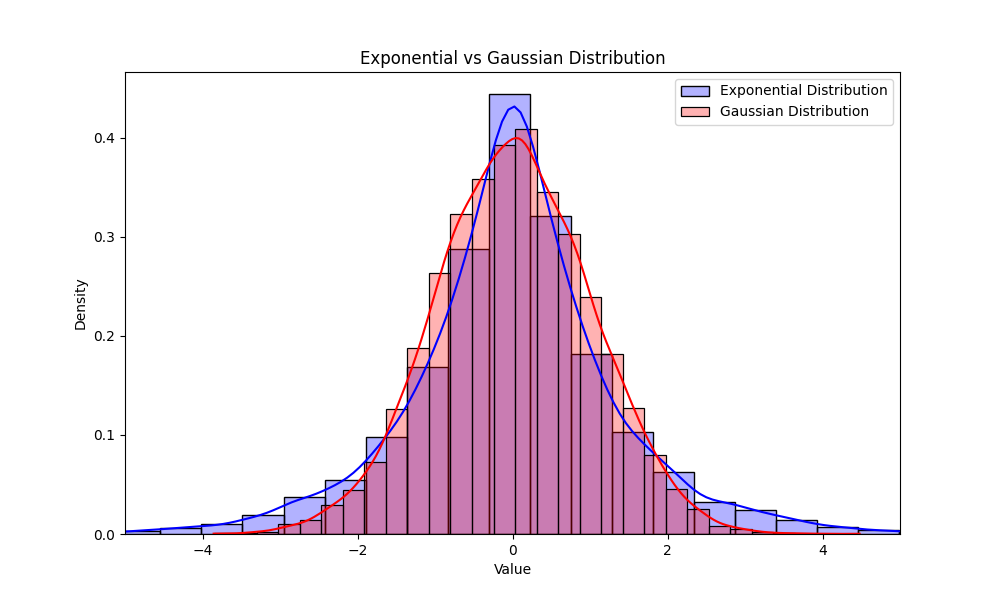
\includegraphics[width=1\textwidth]{imgs/exponential_gaussian_dist.png}
\caption{Comparison of the Gaussian and exponential distribution. The exponential function has a heavier tail and therefore greater exploration capability. The Gaussian function has greater exploitation capability as more probability mass is located around the mean.} \vspace{-1em}
\label{fig:ccc}
\end{figure}
Through the specific modelling of the characteristic length $L^i_{k\Delta t}$ in equation \eqref{qcbo:length} we achieve the same scaling as in the standard CBO.

The update rule \eqref{qcbo:update} together with exponential noise leads us to the following algorithm:

\begin{algorithm}[H]
    \caption{Consensus-based Optimization Algorithm with Exponential Noise}
    \SetAlgoLined
    \KwIn{Population size $N$, time steps $K$, time step length $\Delta t$, consensus weight $\alpha$, exploration parameter $\sigma$}
    \KwOut{Near optimal solution}
    Initialize particles $X^i_0$ randomly with a Gaussian distribution \eqref{qcbo:initial}\;
    \For{$k \gets 1$ \KwTo $K-1$}{
    \For{particle $i$}{
    Evaluate fitness $\CE(X^i_{k\Delta t})$ of each particle\;
    Calculate the attractor $\conspoint{\empmeasure{k\Delta t}}$ with \eqref{qcbo:attractor}\;
    Update position $X^i_{(k+1)\Delta t}$ with \eqref{qcbo:update}\;
    }
    }
    Evaluate fitness $\CE(X^i_{K\Delta t})$ of each particle\;
    Output best solution\;
\end{algorithm}

\section{Integration into CBXpy and runner implementation}
The CBO algorithm with exponential noise is integrated into CBXpy by writing a custom noise sampler that can then be used in several Particle Dynamics tasks like CBO, but for example Consensus-based Sampling, PolarCBO, and others.
The custom noise sampler is an exponential sampler with a random sign assigned to the output.

Code snippets of the integration can be found in Figure \ref{fig:noise} showing the implemented code. \\
To run large-scale experiments, we also implemented an experiment runner suite and visualizations. Several code snippets of this runner can be found in Figures~\ref{fig:runner1}, \ref{fig:runner2}, \ref{fig:runner3}. In Figure \ref{fig:result} a key code snippet for the loading of the results is depicted and in Figure \ref{fig:visualize} one of the many visualization functions is depicted - here for heatmaps in subplots.


\begin{figure}[!ht]
\centering
\subcaptionbox{\footnotesize\label{fig:noise1} The implementation of the exponential noise sampler using numpy.}{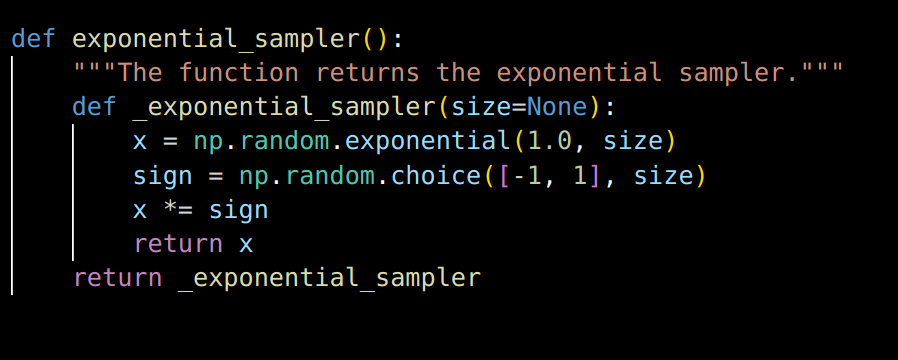
\includegraphics[width=0.45\textwidth]{imgs/noise_numpy}}
\hspace{3em}
\subcaptionbox{\footnotesize\label{fig:noise2} The implementation of the exponential noise sampler using torch.}{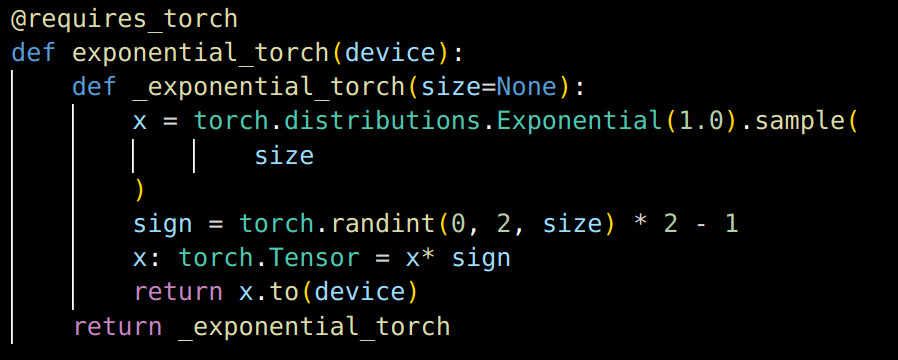
\includegraphics[width=0.45\textwidth]{imgs/noise_torch}}
\caption{The sampler can be used to create a isotropic, anisotropic or covariance noise that behave differently in each dimension. Those noises can then be used to created different versions of all the particle dynamics algorithms like CBO, CBS, PolarCBO.} \vspace{-1em}
\label{fig:noise}
\end{figure}

\section{Numerical Experiments}
In this section, we present numerical experiments to compare the performance of the CBO algorithm with exponential noise with the standard CBO algorithm (with Gaussian noise).
To run large-scale experiments, an experiment runner was written which hyperparameter settings could be set by using .yaml files. It automatically saves the results into an .csv file, that can then be used by various visualization functions to draw information from the results.
In the experiments, mainly the optimization of the Rastrigin function is considered. Its parameter space is thoroughly tested to compare the CBO with Gaussian and exponential noise. The Rastrigin function is a non-convex function with many local minima and a global minimum at the origin. We compare the performance of the CBO algorithm with exponential noise and Gaussian noise in terms of the convergence rate and the quality of the solutions found. The success factor is defined as the percentage of runs in which the algorithm finds a function value below the second best minima.

\subsection{Mean-Field behaviour}
The first question that arises is how the algorithm behaves in the mean-field limit. Fornasier, Klock and Riedl explored in their paper "Convergence of Anisotropic Consensus-Based
Optimization in Mean-Field Law" the convergence of the CBO method and found an exponential convergence in the mean-field. This rate is independent of the dimensionality of the problem. The result for the CBO with Gaussian noise could be confirmed with own experiments and can be seen in Figure \ref{fig:meanfield}.
For CBO with exponential noise we take the same parameters and try to find a similar correlation. As it turns out, even with exponential noise, the mean-field convergence stays on its exponential trend with almost the same convergence rate of $\exp(-0.94(2\lambda-\sigma^2) t)$. 
% ((MAYBE: ?? Still not sure: This can be explained by the central limit theorem. It states that the distribution will tend toward a Gaussian distribution always as the number of variables (what are the variables here?) increases, regardless of the original distribution, provided the original distributions have finite mean and variance.))

\begin{figure}[!ht]
\centering
\subcaptionbox{\footnotesize\label{fig:cbo_meanfield} The mean-field behaviour of CBO with Gaussian noise.}{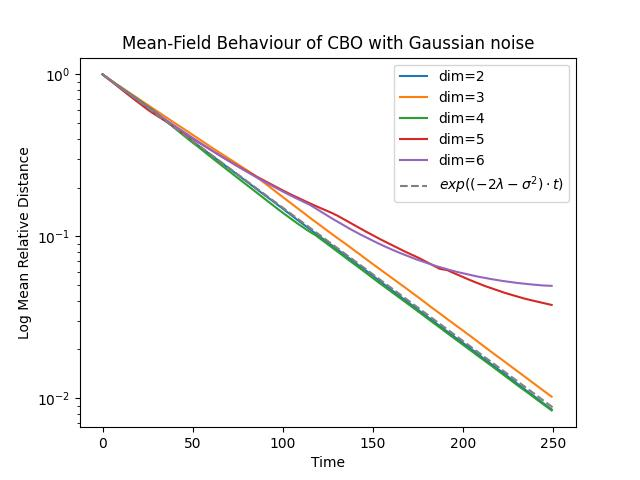
\includegraphics[height=4.6cm, width=0.4\textwidth]{imgs/cbo_meanfield_anisotropic}}
\hspace{3em}
\subcaptionbox{\footnotesize\label{fig:qcbo_meanfield} The mean-field behaviour of CBO with exponential noise.}{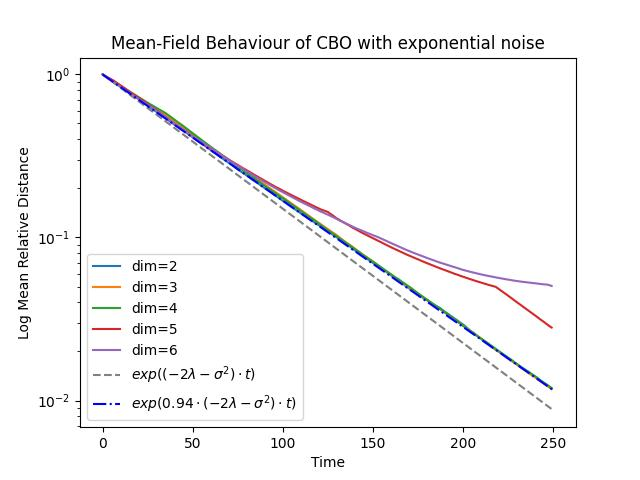
\includegraphics[height=4.6cm, width=0.4\textwidth]{imgs/qcbo_meanfield_anisotropic}}

\caption{A depiction of the mean-field behaviours of CBO with Gaussian and exponential anisotropic noise. For the Rastrigin function~$\CE(v)\!=\!\sum_{k=1}^d \!v_k^2\!+\!\frac{5}{2}(1\!-\!\cos(2\pi v_k))$ with~$\globmin \!=\! 0$ and several local minima, we evolve the discretized system of isotropic and anisotropic CBO using $N = 10000$ particles, discrete time step size~$\Delta t = 0.01$ and \mbox{$\alpha = 10^{15}$}, $\lambda = 1$, and $\sigma = 0.32$ for different dimensions~$d\in\{2,3,4,5,6\}$.
We observe in both cases that the convergence rate of the energy functional~$\CV(\empmeasure{t})$ is independent from $d$ and lies at around $(2\lambda-\sigma^2)$. However, the {\color{red}guess her sth is missing}} \vspace{-1em}
\label{fig:meanfield}
\end{figure}


% How does QCBO and CBO behave in the mean-field?
% SUMMARY 8
% Wie in Email von Konstantin also verschiedene Sigmas 
% und dimensionen

\subsection{Hyperparameter Performance with different Dimensionality}
To thoroughly study the hyperparameter settings and differences for CBO with Gaussian and exponential noise several experiments with different lambda and sigma values are created. This subsection should give an insight into how success probability depends on their relationship of the method with different dimensions of the objective function. As you can see in the Figure \ref{fig:d_sigma_lambda}, both CBO with Gaussian and exponential noise become very sensitive to the hyperparameter setting. It can be seen that CBO with exponential noise needs a not as high sigma as the CBO with Gaussian noise. That was as expected, as the exponential noise has more probability mass on its tails leading to greater exploration capabilities of the CBO algorithm.

\begin{figure}[!ht]
\centering
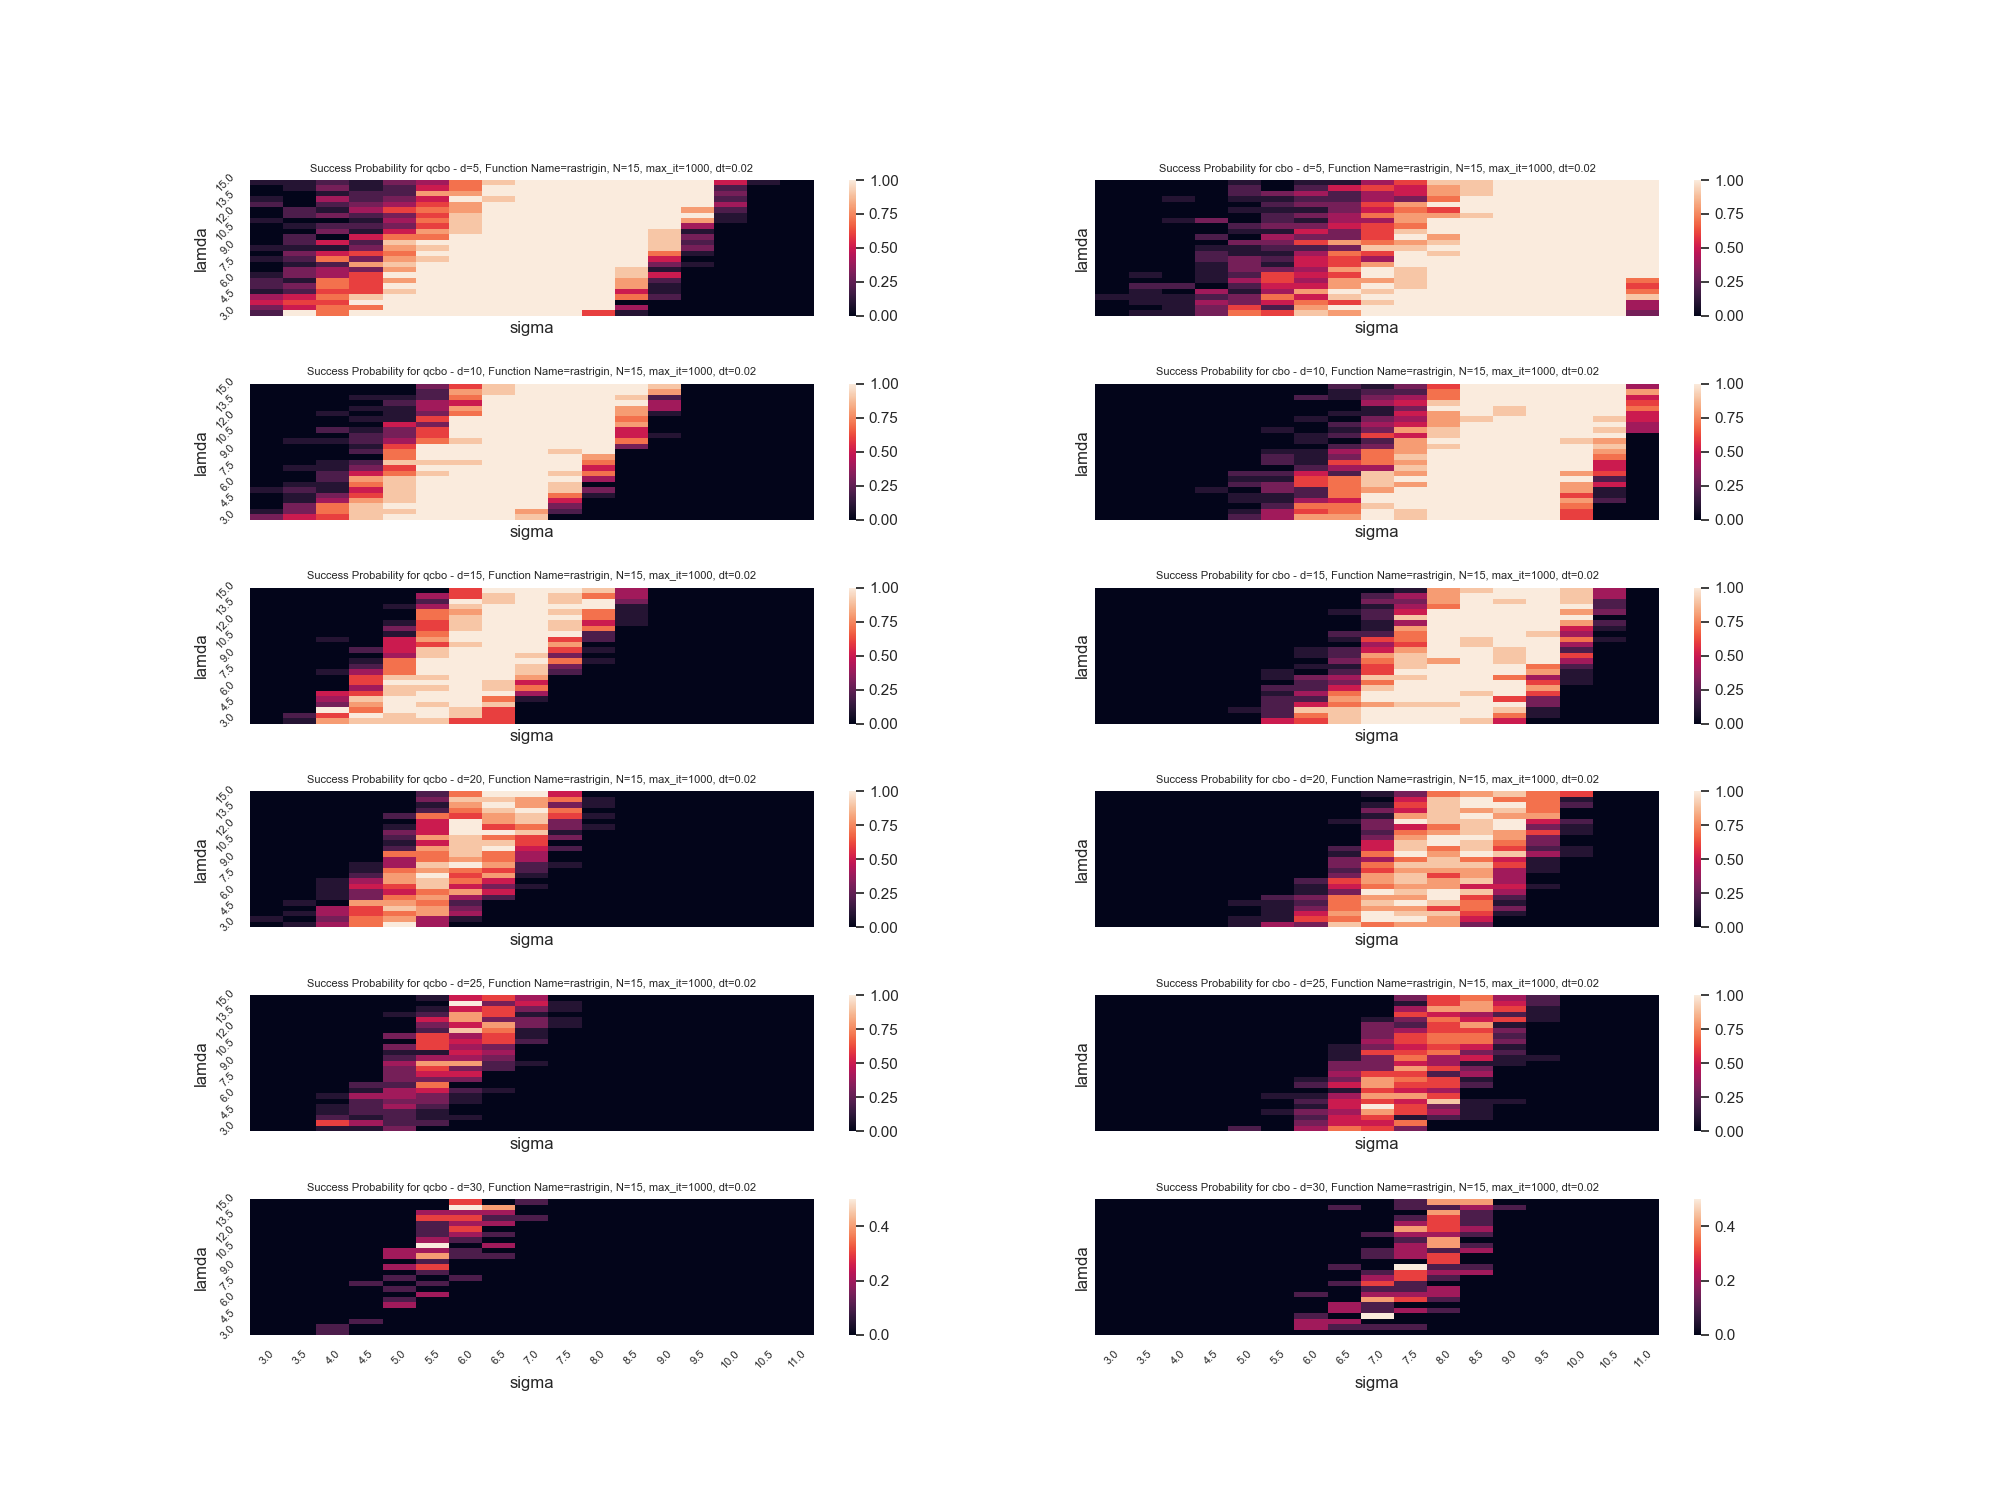
\includegraphics[width=1\textwidth]{imgs/d_sigma_lambda.png}

\caption{A demonstration of the increased sensitivity of hyperparameter settings with increased dimensionality. On the left side the CBO is depicted, on the right side the QCBO. Both are evaluated with $d=5,10,15,20,25,30$.} \vspace{-1em}
\label{fig:d_sigma_lambda}
\end{figure}

% The tightening of the feasible hyperparameter space in the QCBO and CBO method. They have different convergent hyperparameters
% SUMMARY 8

\subsection{Hyperparameter Performance with different Alpha values}
In this subsection the influence of the alpha values is investigated. The alpha value controls the weight of the consensus point in the CBO algorithm with exponential noise. It does not impact the hyperparameter sensitivity of neither the CBO with Gaussian noise nor the CBO with exponential noise as the Figure \ref{fig:alpha_sigma_lambda} shows. 

\begin{figure}[!ht]
\centering
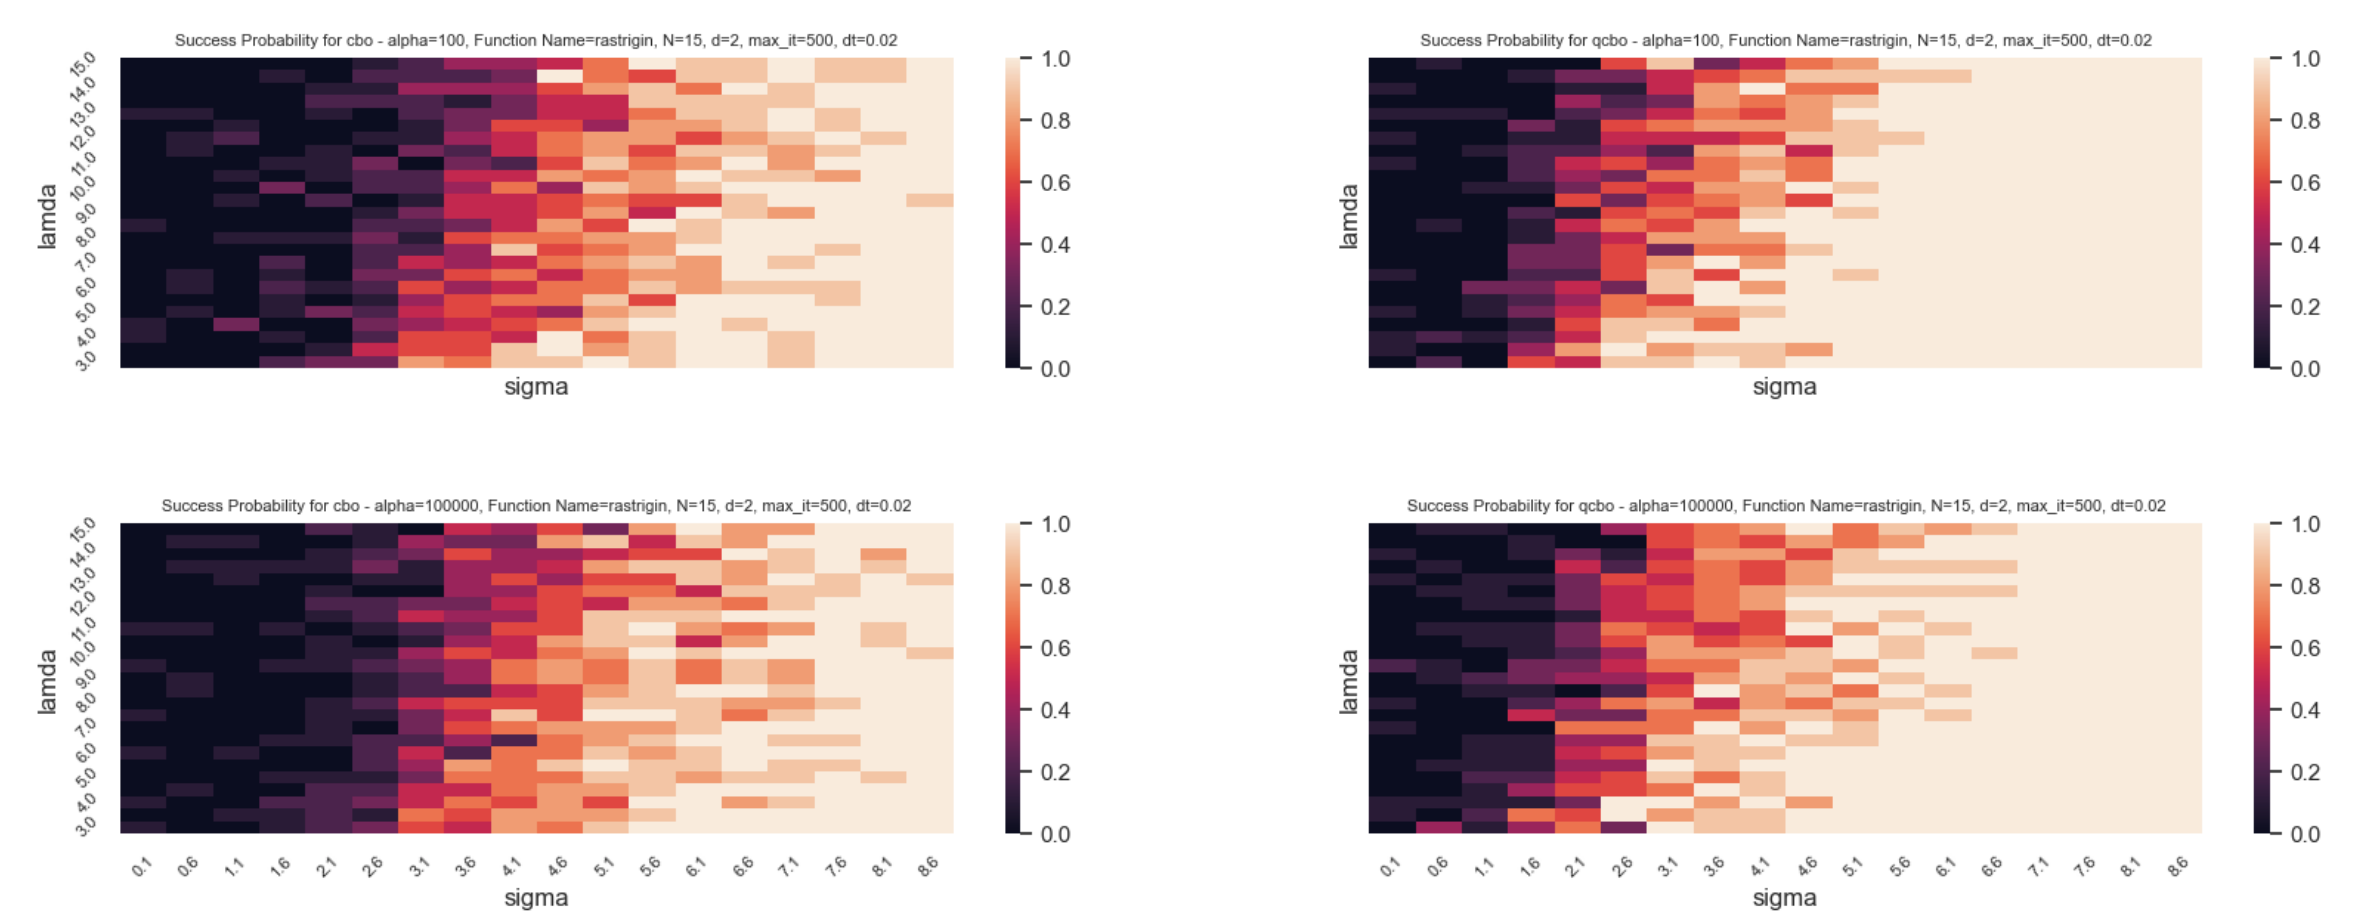
\includegraphics[width=1\textwidth]{imgs/alpha_sigma_lambda.jpg}

\caption{The Figure captures the differences in the success probability with different hyperparameter settings of $\lambda$ and $\sigma$ observed at different values of $\alpha$. Both dynamics are evaluated at $alpha = 100, 10000$.} \vspace{-1em}
\label{fig:alpha_sigma_lambda}
\end{figure}

% Not so much difference here. Neither in QCBO or CBO.
% SUMMARY 8
% Alpha is the parameter that controls the weight of the consensus point in the CBO algorithm with exponential noise. We investigate the effect of different alpha values on the performance of the CBO algorithm with exponential noise.

\subsection{Hyperparameter Performance with different number of particles}
Another experiment that has been conducted is to map the relationship between the the number of particles, sigma and lambda. Plotting sigma on the x-axis and the number of particles on the y-axis, we recognize a probability distribution with quadratic contour arises when using the CBO with exponential noise. This probability distribution is then linearly shifted along the x-axis with changing lambda values. The same happens with the CBO with Gaussian noise - even if the distribution contours seem far broader than the CBO exponential one. This can be seen in Figure \ref{fig:cbo_n_sigma_lambda} for CBO with Gaussian noise and in Figure \ref{fig:qcbo_n_sigma_lambda} for CBO with exponential noise. The more narrow probability distribution than the CBO with Gaussian noise indicates a higher sensitivity to hyperparameters.

\begin{figure}[!ht]
\centering
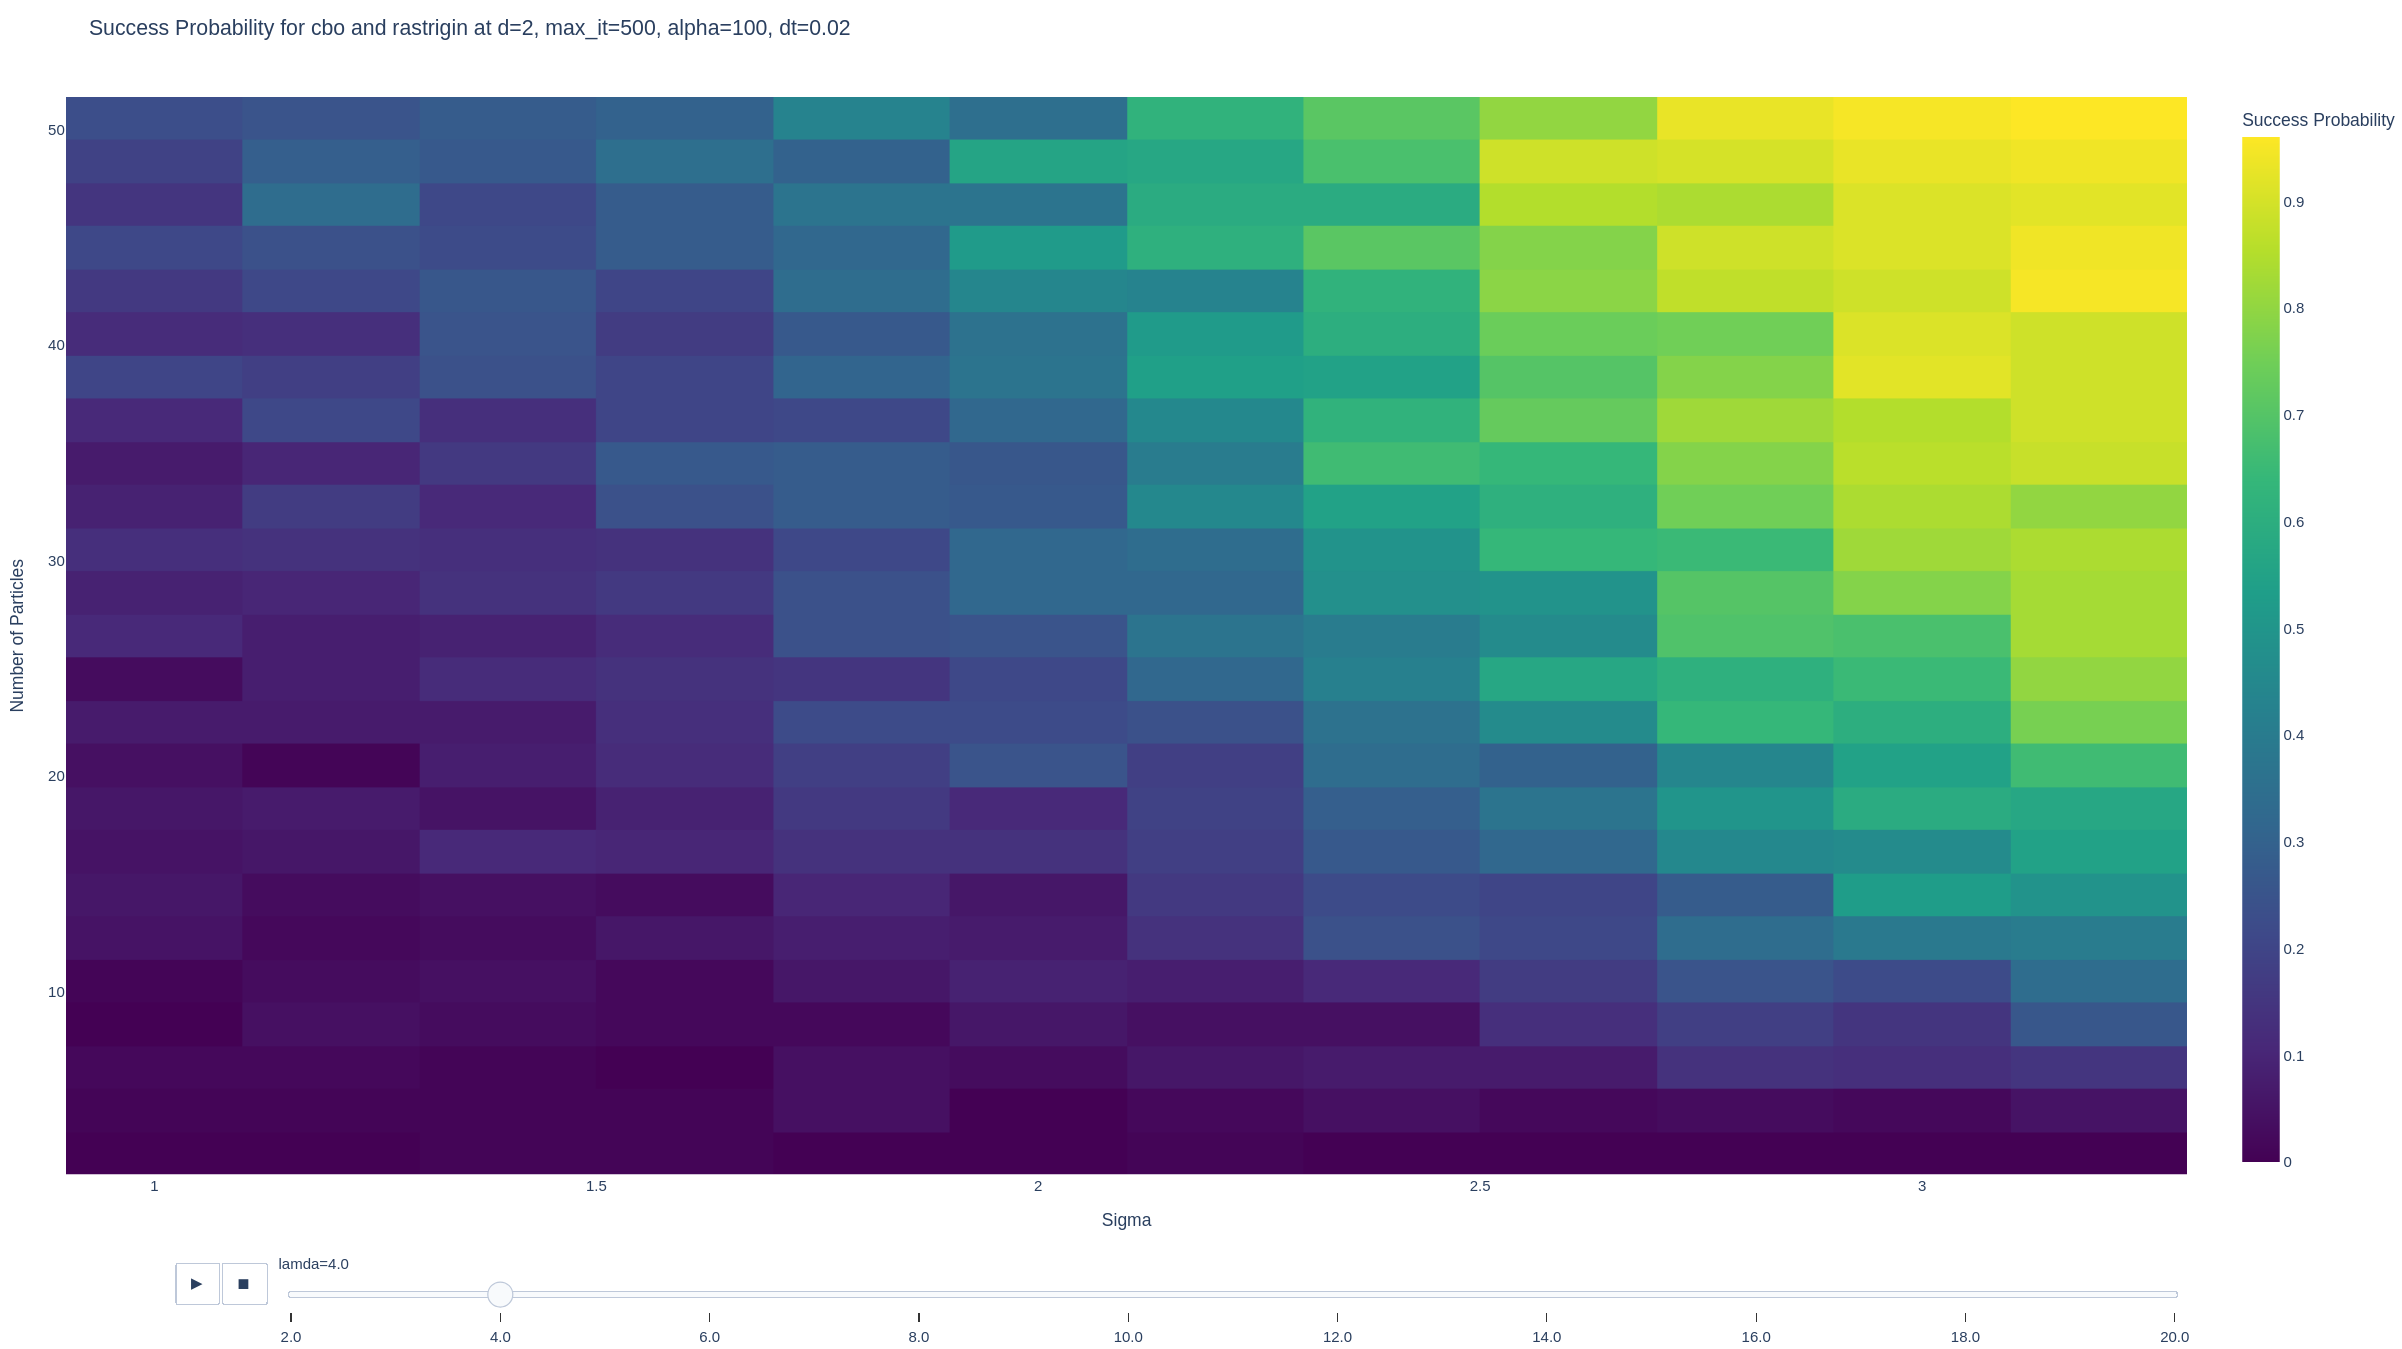
\includegraphics[width=1\textwidth]{imgs/cbo_n_sigma_lambda.png}

\caption{CBO with Gaussian noise: It is apparent that the higher the sigma and the higher the lambda, the higher the success probability} \vspace{-1em}
\label{fig:cbo_n_sigma_lambda}
\end{figure}
\begin{figure}[!ht]
\centering
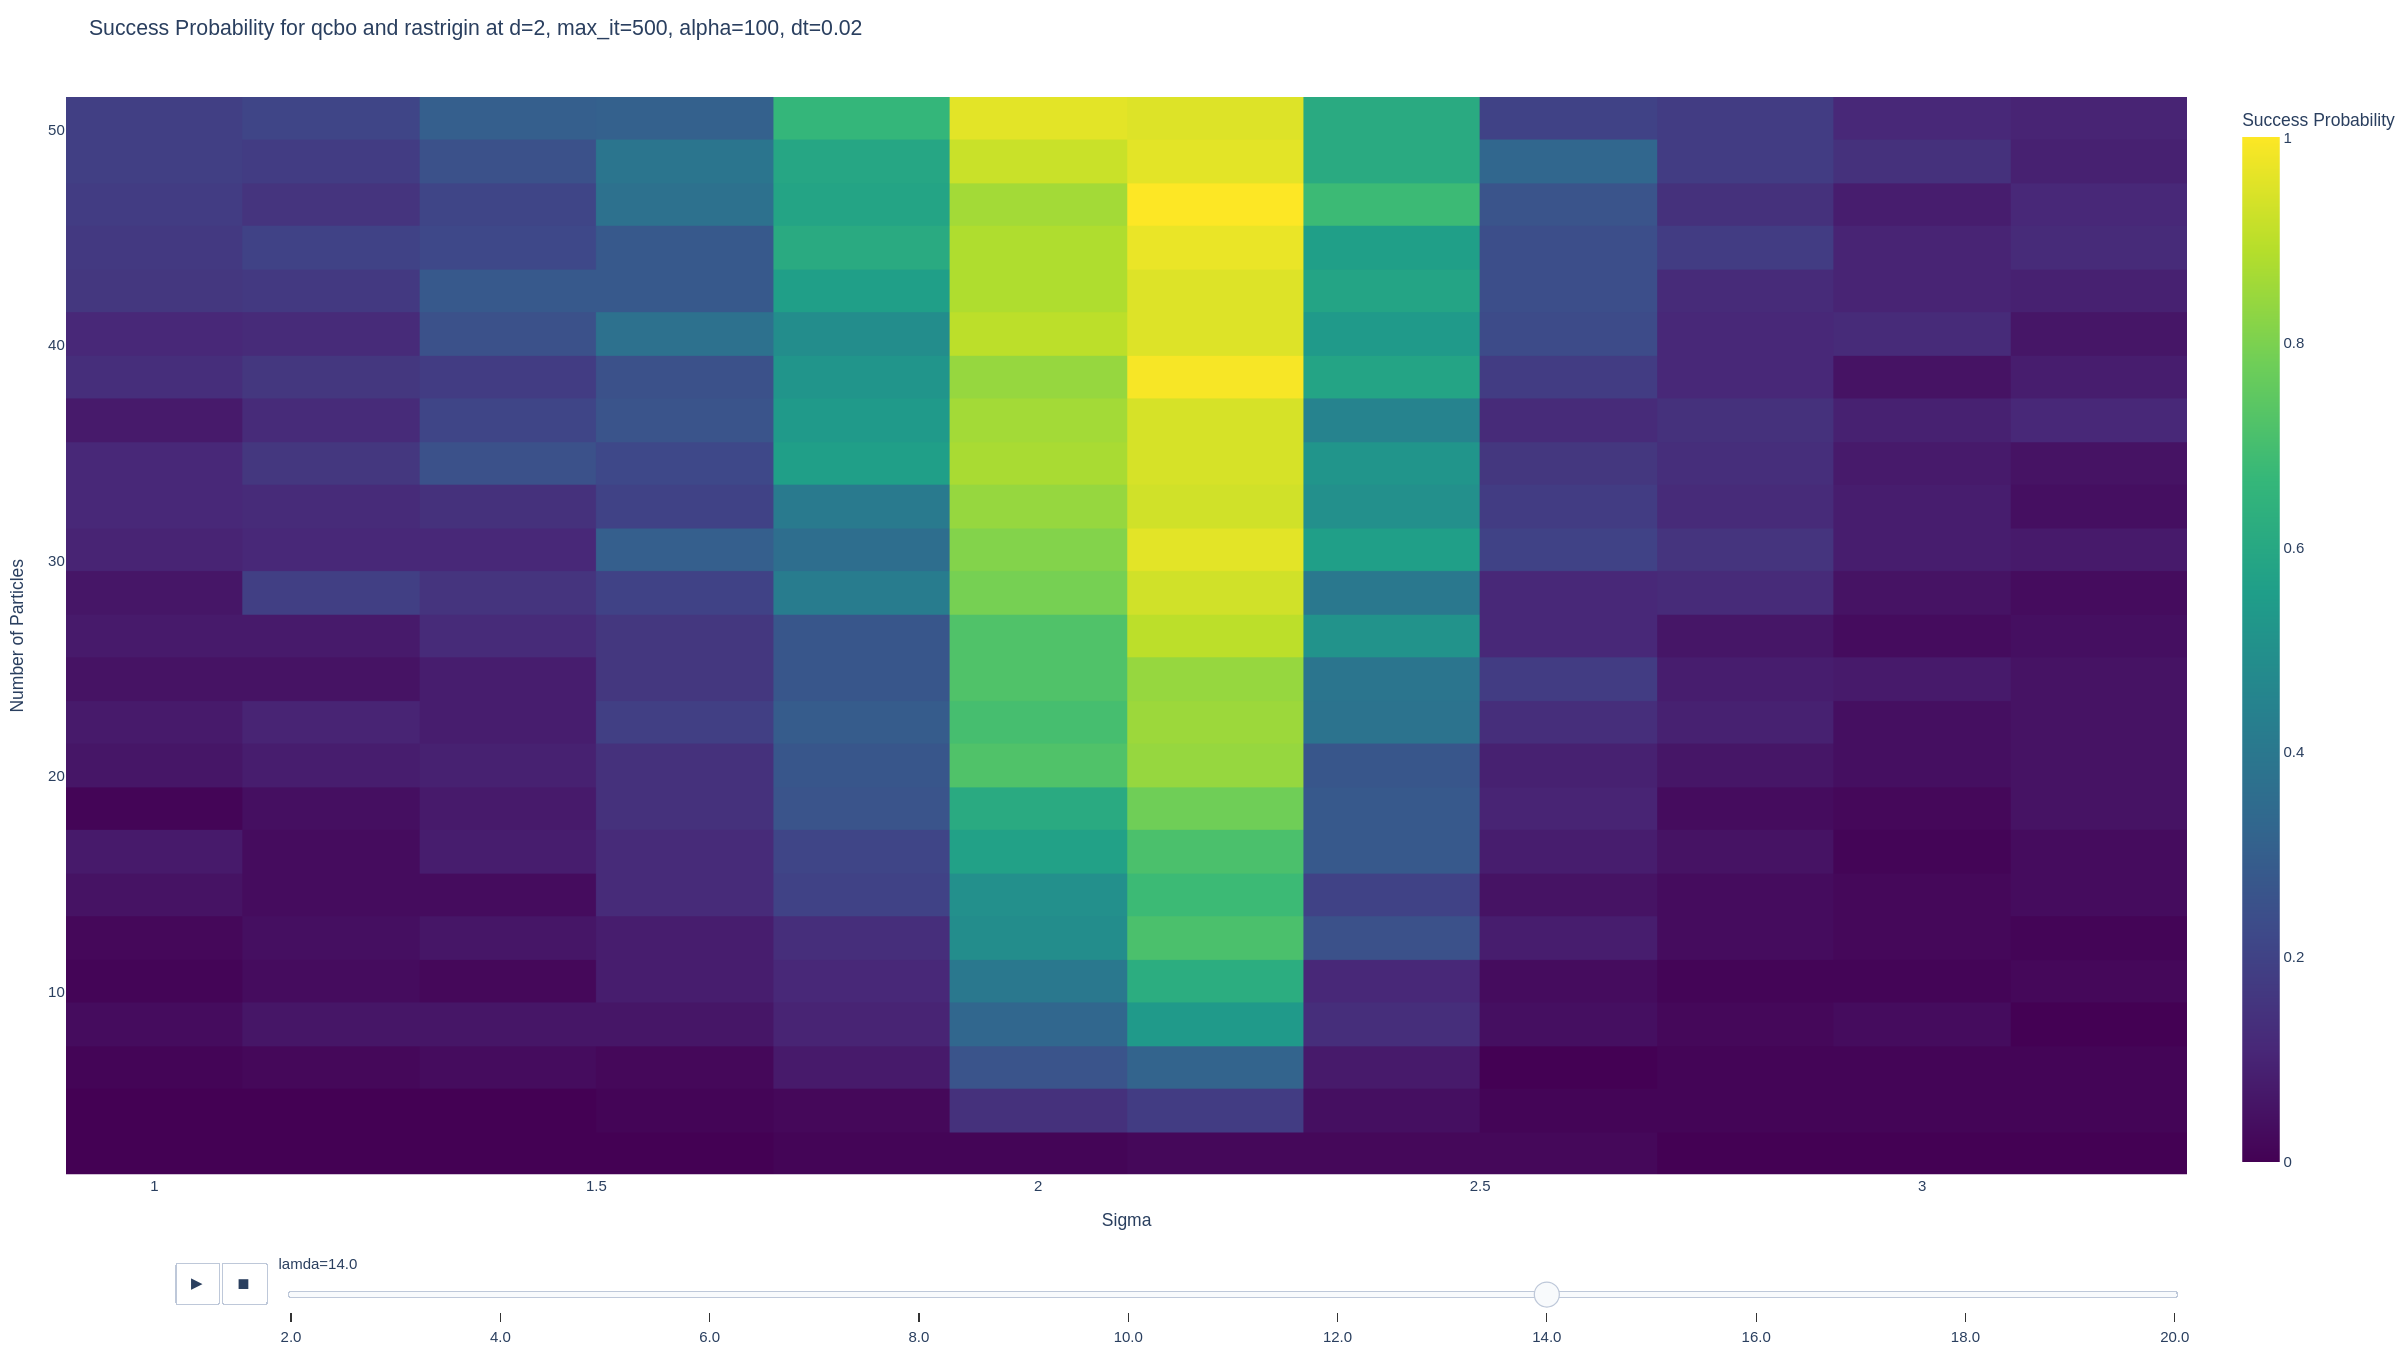
\includegraphics[width=1\textwidth]{imgs/qcbo_n_sigma_lambda.png}

\caption{For CBO with exponential noise, we see a higher sensitivity to the hyperparameter settings than in the CBO with Gaussian noise.} \vspace{-1em}
\label{fig:qcbo_n_sigma_lambda}
\end{figure}


% As there is a relationship between the number of particles, lambda and sigma that 
% 3D plots show a linear correlation between the maximum/probability distribution in the sigma N plot with the lambda value chosen.
% SUMMARY 6

\subsection{Real-world Machine Learning Applications}
We see that CBO and QCBO behave fairly similar when optimizing the machine learning landscape of a neural network with one hidden layer for the MNIST dataset. The model used is a multi-layer perceptron with a hidden layer of 100 neurons, 1D batch normalization, and cross entropy loss. The experiment shows that the heavy-tailed noise does not have much influence on the exploitation capability needed in neural network optimization. The diagram showing the accuracy over epochs can be seen in Figure \ref{fig:mnist}. 

\begin{figure}[!ht]
\centering
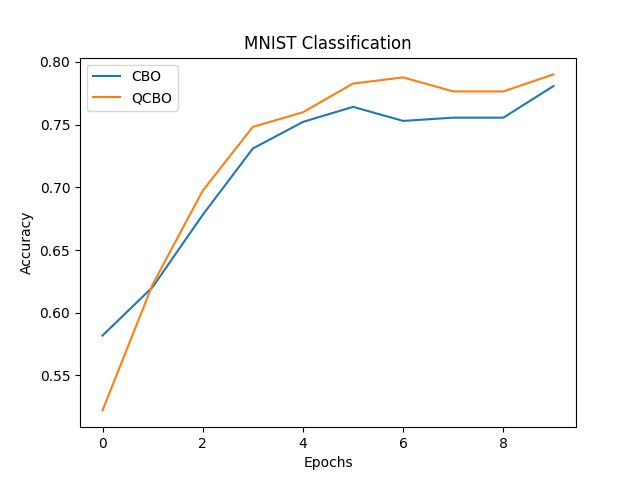
\includegraphics[width=1\textwidth]{imgs/mnist.png}

\caption{It can be observed that CBO with exponential noise works similar on a neural network optimization as the one with Gaussian noise. For both, the same parameters were used: $\alpha = 50.0$, $\Delta t = 0.1$, $\sigma = 0.1$, $\lambda = 1.0$, $max\_it = 200$} \vspace{-1em}
\label{fig:mnist}
\end{figure}

\section{Interpretation and Discussion}
Integrating exponential noise into the CBO algorithm has shown similar results as the CBO algorithm with Gaussian noise. Our tests show that CBO with exponential noise maintains almost the same strong convergence rate as with Gaussian noise in the mean-field limit. This suggests that using exponential noise does not affect the ability of the algorithm to converge. 
One of the key takeaways is that CBO with exponential noise has similar behaviour during the optimization process. Even though the hyperparameter settings are naturally different, Gaussian and exponential noise sigma and lambda interactions take the same forms across different number of dimensions and alpha values.
% requires a smaller sigma value compared to Gaussian noise, meaning it can explore the solution space more efficiently while using less noise. This could be useful in high-dimensional problems where the balance between exploration and exploitation is important.

In practical applications, such as optimizing neural networks, both noise models performed similarly. It shows that exponential noise does not hinder the algorithm’s ability to exploit promising solutions but improves exploration without sacrificing accuracy.

In the future, it would be interesting to explore how exponential noise performs in more complex optimization problems and across different machine learning models.

\clearpage

\bibliographystyle{abbrv}
\bibliography{biblio.bib}

\clearpage
\section*{Additional Figures}
\begin{figure}[!ht]
\centering
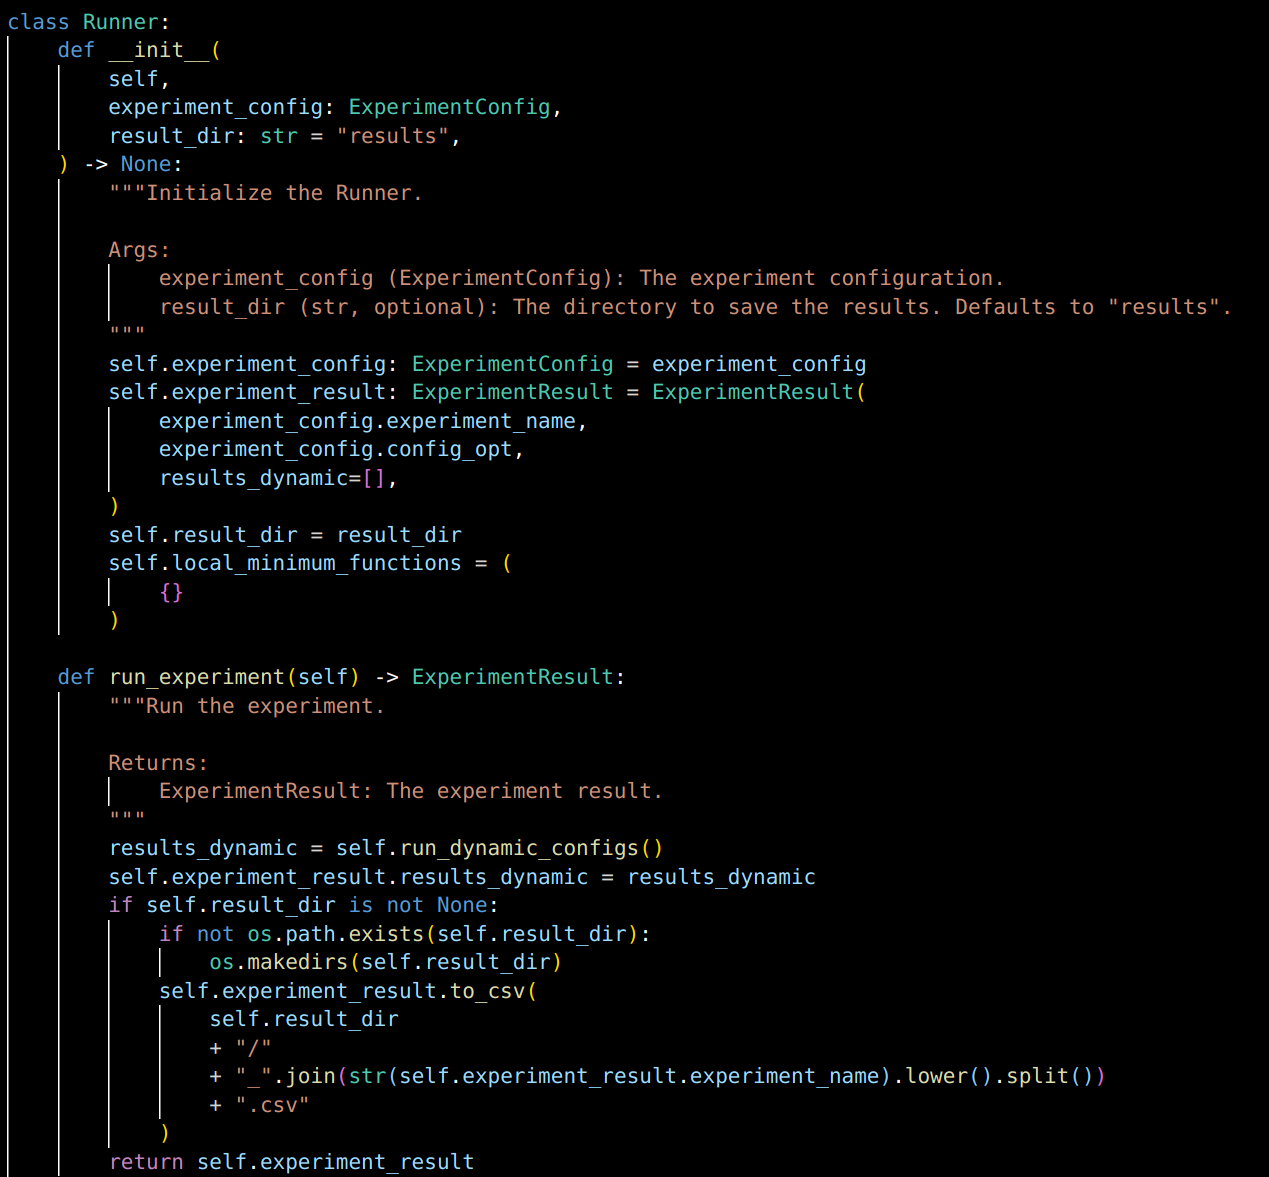
\includegraphics[width=1\textwidth]{imgs/runner1.png}
\caption{The runner class initializes large-scale experiments for by loading an ExperimentConfig that was obtained from .yaml files. The function $run\_experiment$ is responsible for running all the different configurations and saving it as a ExperimentResult.} \vspace{-1em}
\label{fig:runner1}
\end{figure}

\begin{figure}[!ht]
\centering
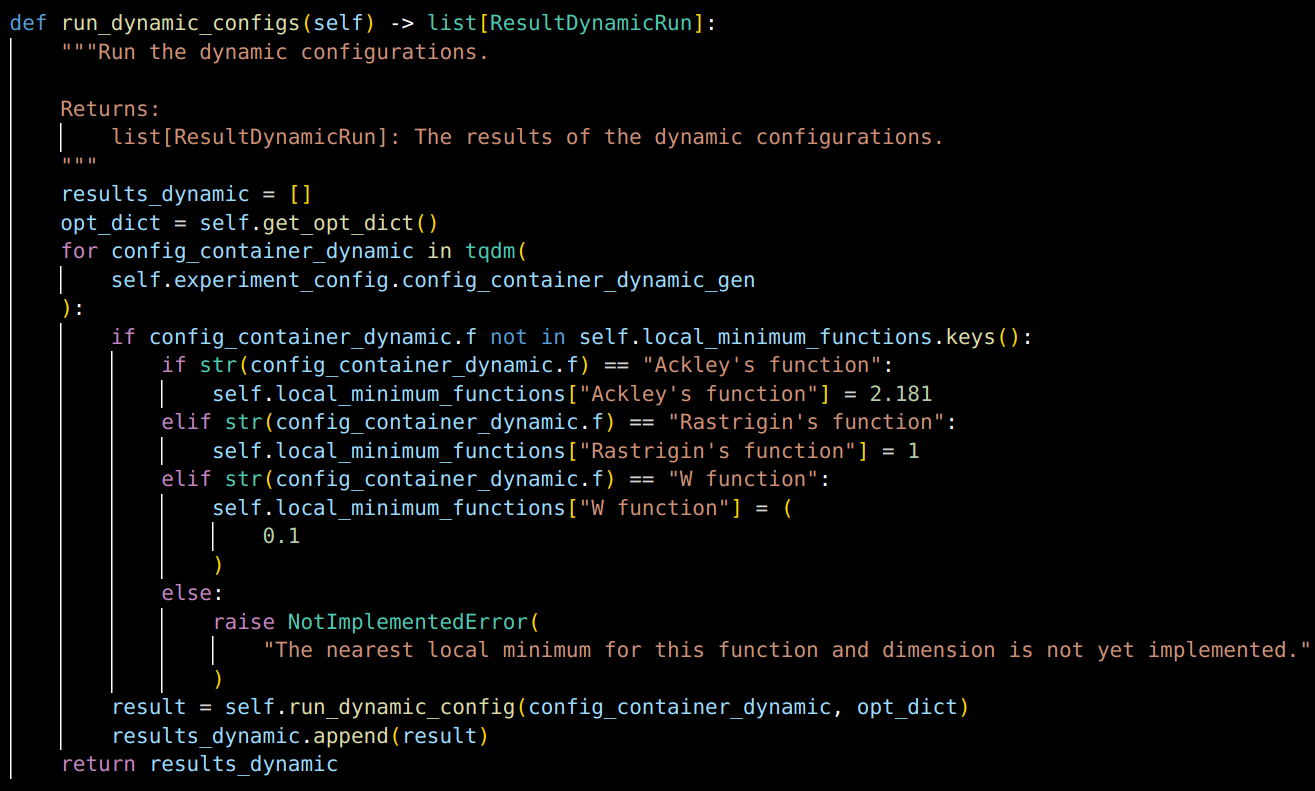
\includegraphics[width=1\textwidth]{imgs/runner2.png}
\caption{The $run\_dynamic\_configs$ function runs all configurations and before includes the second-best minima objective energy values.} \vspace{-1em}
\label{fig:runner2}
\end{figure}

\begin{figure}[!ht]
\centering
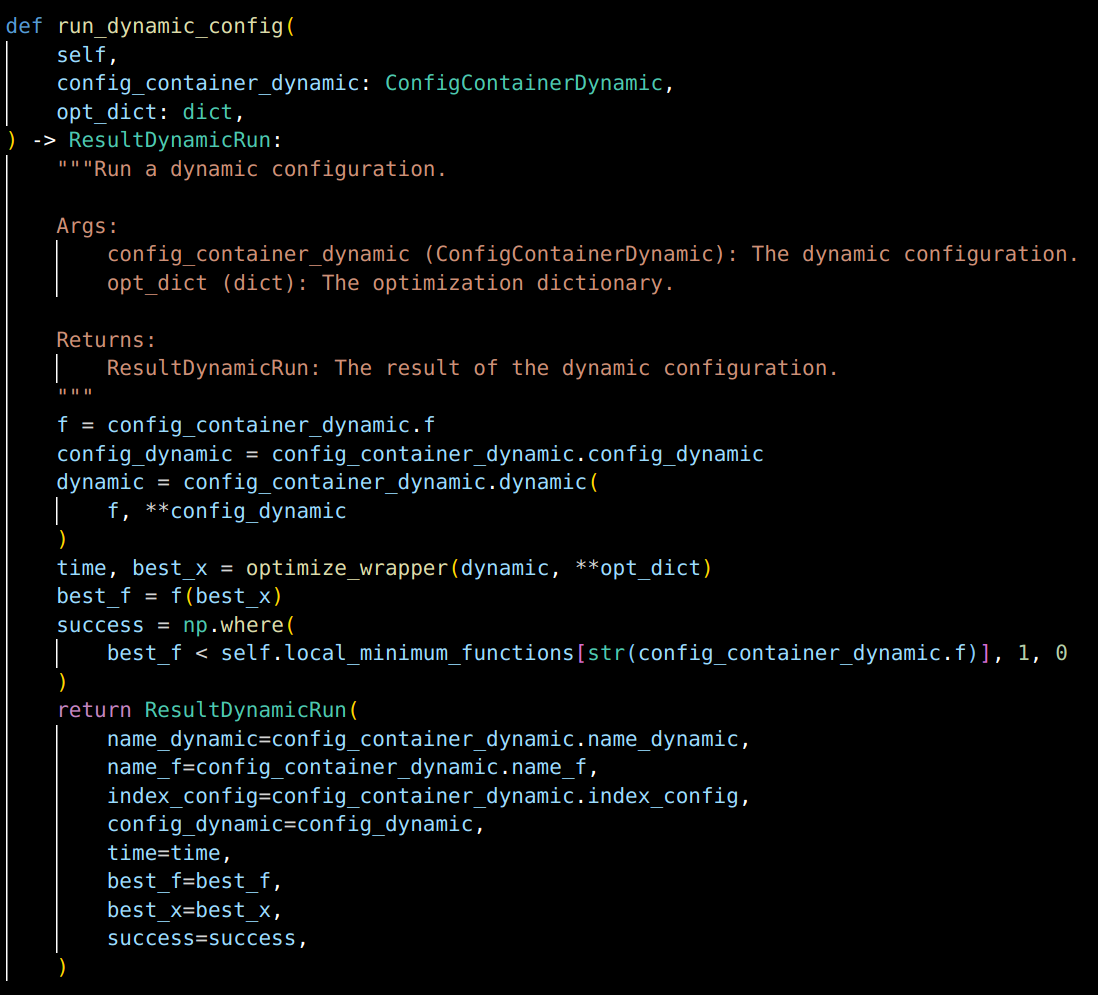
\includegraphics[width=1\textwidth]{imgs/runner3.png}
\caption{The $run\_dynamic\_config$ runs one configuration and gives out the result.} \vspace{-1em}
\label{fig:runner3}
\end{figure}

\begin{figure}[!ht]
\centering
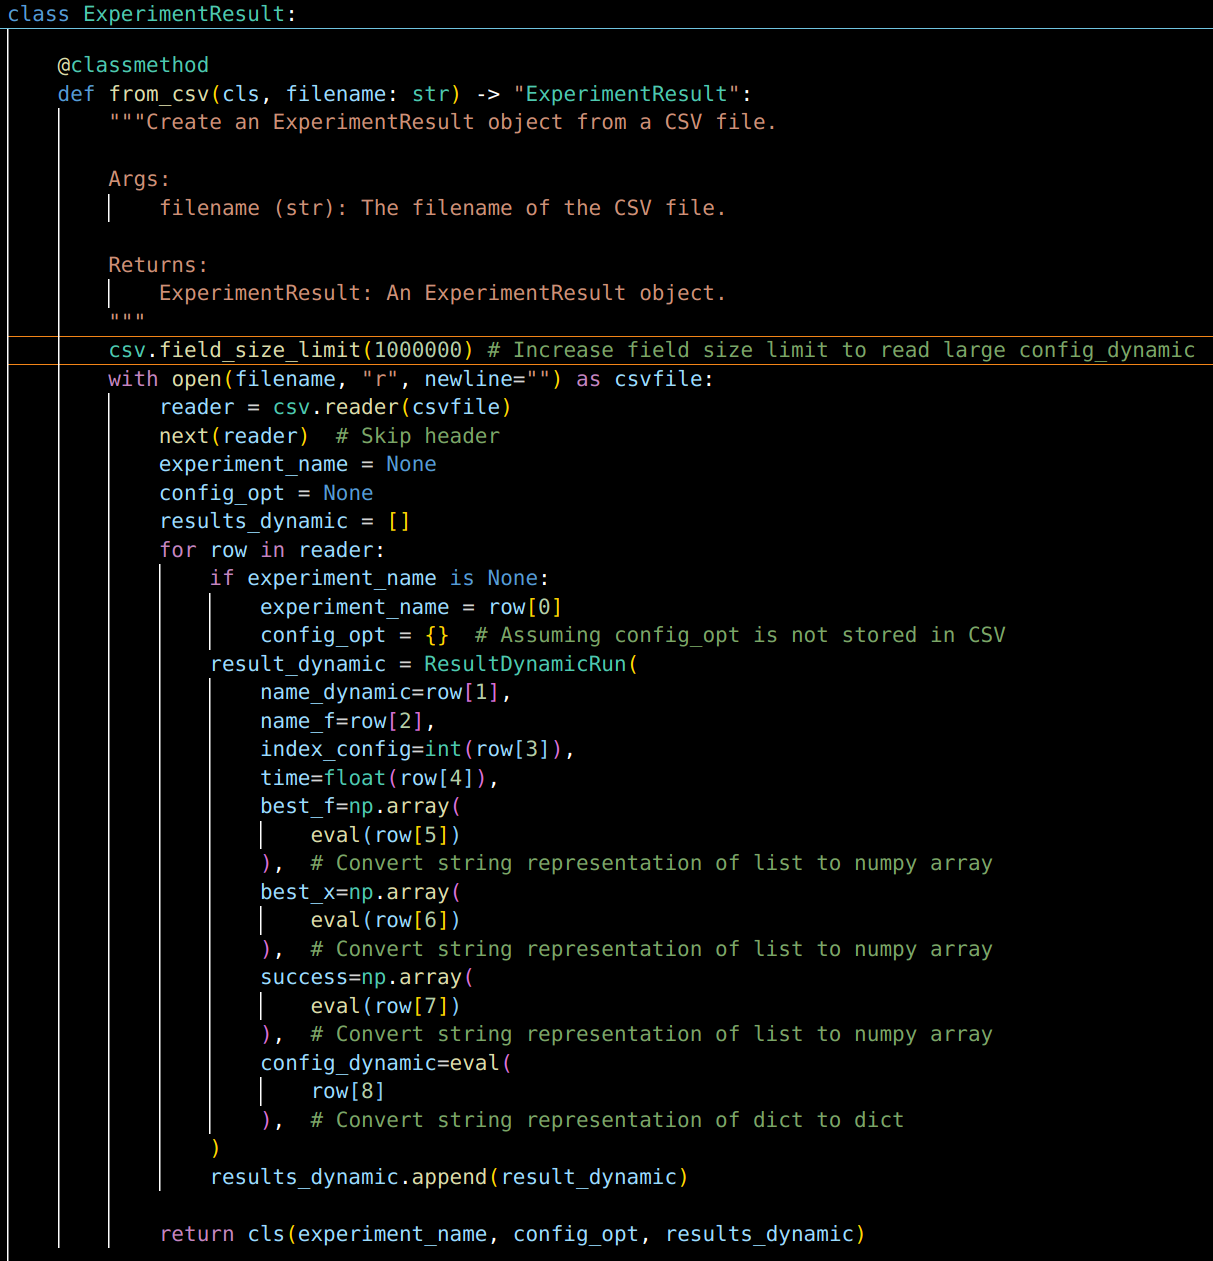
\includegraphics[width=1\textwidth]{imgs/result.png}
\caption{This class is responsible for saving and loading results.} \vspace{-1em}
\label{fig:result}
\end{figure}

\begin{figure}[!ht]
\centering
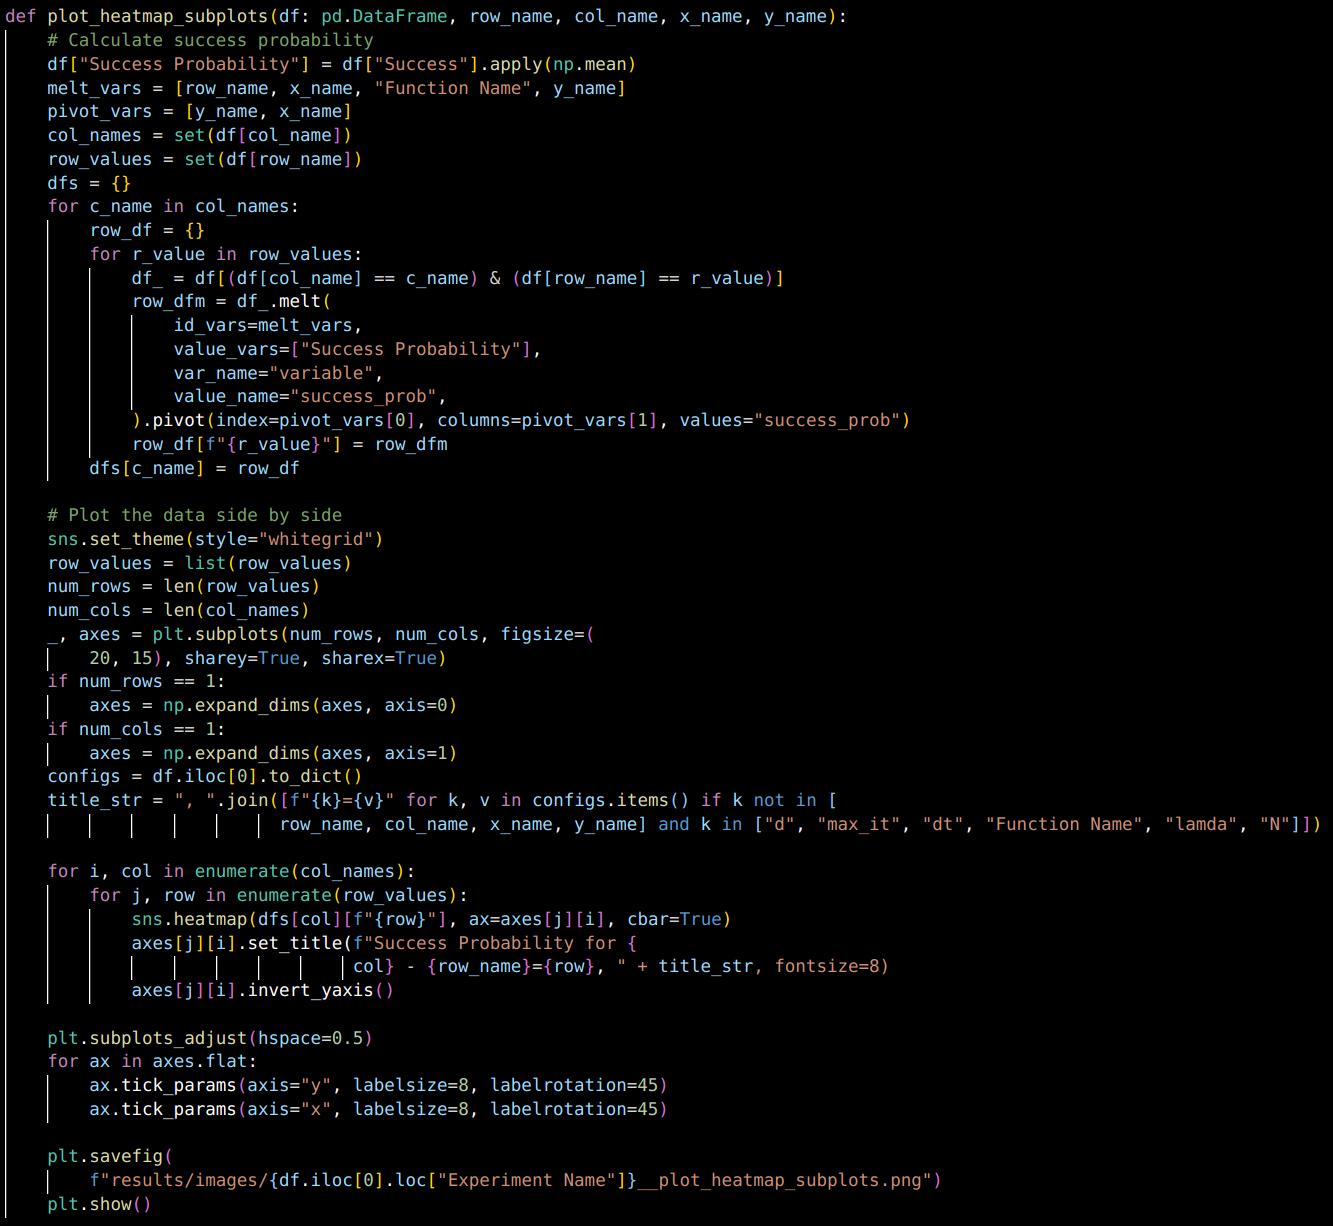
\includegraphics[width=1\textwidth]{imgs/visualize.png}
\caption{This function generates heatmaps in a subplot.} \vspace{-1em}
\label{fig:visualize}
\end{figure}

\begin{figure}[!ht]
\centering
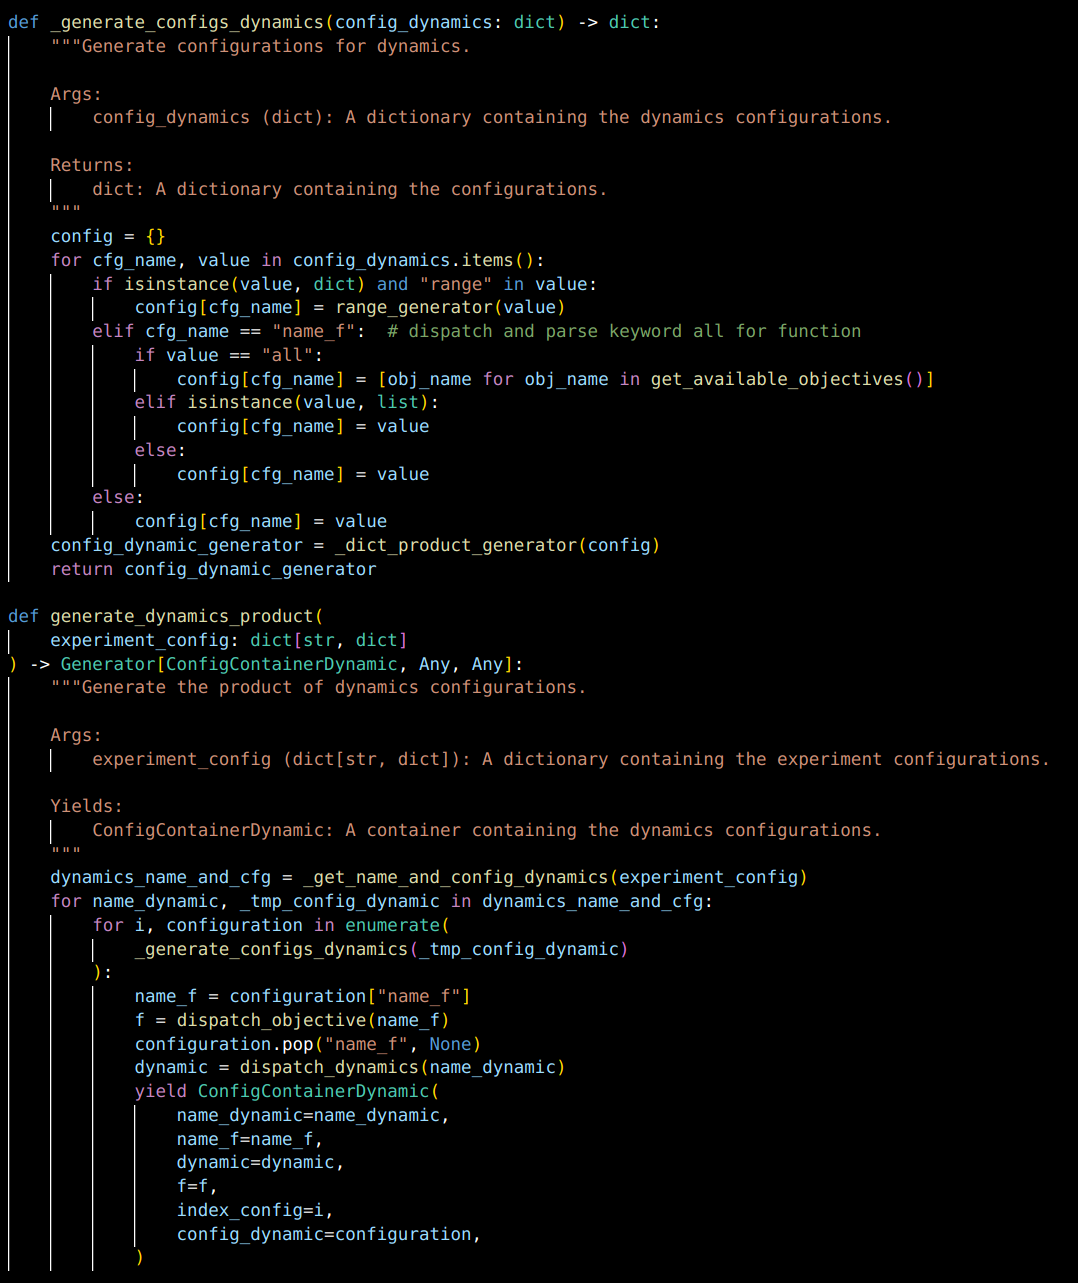
\includegraphics[width=1\textwidth]{imgs/experimentgeneration.png}
\caption{Those two functions are the main responsible ones for converting a .yaml file into a generator of experiment configurations.} \vspace{-1em}
\label{fig:experimentgeneration}
\end{figure}

\end{document}
